\documentclass[11pt,letterpaper,oneside]{phstylee}

\usepackage[mathscr]{eucal}
\usepackage[table]{xcolor}
\usepackage{makeidx}
%\usepackage[ansinew]{inputenc}
%\usepackage[latin1]{inputenc}
\usepackage[final]{pdfpages}
\usepackage[utf8x]{inputenc}
\usepackage[spanish,es-noquoting]{babel}
\usepackage{array}
%\usepackage{epsfig}
%\usepackage{psfig}
%\usepackage{subfigure}
%\usepackage[dvips]{graphicx}
\usepackage{cite}
\usepackage{amsfonts}
\usepackage{amsmath}
\usepackage{amssymb}
\usepackage{amsxtra}
\usepackage{varioref}
\usepackage{multicol}
\usepackage{float}
\usepackage{rotate}
\usepackage{rotating}
\usepackage{color}
\usepackage{enumerate}
\usepackage{pmat}
%\usepackage{theorem}
%\usepackage[pdftex]{graphicx}
\usepackage{graphicx}
%\usepackage{hangcaption}
\usepackage{latexsym}
%\usepackage{stmaryrd}
% \usepackage{euler}
\usepackage{amsthm}
\usepackage{dsfont}
\usepackage{epstopdf}
%\epstopdfsetup{outdir=.}
\DeclareGraphicsExtensions{.pdf,.png,.jpg}
\usepackage{caption}
\usepackage{subcaption}
\usepackage{multirow}
\setcounter{secnumdepth}{5}
\usepackage{algorithm}
\usepackage{algpseudocode}

%\usepackage{fancybox}
%\usepackage{hyperref}
%\usepackage[pdftex,bookmarks,colorlinks]{hyperref} 
%\hypersetup{colorlinks,linkcolor=blue,urlcolor=blue}
%%%%%%%%%%%%%%%%%%%%%
%      DIRECTORIO DONDE BUSCA LAS FIGURAS

\graphicspath{{img/}}
\usepackage{pifont}
\usepackage{textcomp}
\usepackage{subcaption}
\usepackage{pgf}
\usepackage{tikz}
\usepackage{listings}
\usepackage{afterpage}
\usepackage[normalem]{ulem}
\usetikzlibrary{shapes,arrows,positioning,calc,shadows}

\addto\captionsspanish{%
\def\bibname{Referencias}%
\def\tablename{Tabla}%
\def\listtablename{ÍNDICE DE TABLAS}%
\def\listfigurename{ÍNDICE DE FIGURAS}
}

\renewcommand{\listfigurename}{ÍNDICE DE FIGURAS}
\renewcommand{\listtablename}{ÍNDICE DE TABLAS}

\newcommand{\comm}[1]{
\noindent\fbox{\parbox{\textwidth}{\begin{center} #1 \end{center}
}}\\}

\usepackage{mdframed}

\newcommand{\midtilde}{\raisebox{0.5ex}{\texttildelow}}

\usepackage{multirow}
\usepackage{etoolbox}
%\patchcmd{\thebibliography}{\section*{\refname}}{}{}{}

\definecolor{colora}{RGB}{102,190,14}
\definecolor{colorb}{RGB}{174,128,3}
\definecolor{colorc}{RGB}{204,51,51}
\definecolor{colord}{RGB}{174,3,128}
\definecolor{colore}{RGB}{120,14,190}
\definecolor{colorf}{RGB}{30,76,201}

\renewcommand\thesubsubsection{\Alph{subsubsection}}

\addtolength{\topmargin}{-30pt}

\usepackage[colorlinks=false,linkcolor=black,citecolor=black,hidelinks]{hyperref} %Para evitar recuadros de links.
\linespread{1.1}
\makeindex
\spanishdecimal{.}
\allowdisplaybreaks


%%%%% FIXME (set status=final to remove all comments before submitting) %%%%%
\usepackage[footnote, status=draft, nosilent, nomargin]{fixme}
\fxsetup{theme=color, mode=multiuser} 
\FXRegisterAuthor{gc}{agc}{\color{red}Gonzalo's comment}
\FXRegisterAuthor{jg}{ajg}{\color{brown}Jairo's comment}

\usepackage{soul}
\newcommand{\sgcnote}[1]{\gcnote{\color{gray}{\st{#1}}}}
\newcommand{\sjgnote}[1]{\jgnote{\color{gray}{\st{#1}}}}
%%%%%


%%%%%%%%%%%%%%%%%%%%%%%%%%%%%%%%%%%%%%%%%%%%%%%%%%%%%%%%%%%%
%%%%%%%%%%%%%%%%%%%%%%%%%%%%%%%%%%%%%%%%%%%%%%%%%%%%%%%%%%%%

\begin{document}

\tikzset{
block/.style = {draw, fill=white, rectangle, minimum height=3em, minimum width=3em},
tmp/.style  = {coordinate}, 
sum/.style= {draw, fill=white, circle, node distance=1cm},
input/.style = {coordinate},
output/.style= {coordinate},
pinstyle/.style = {pin edge={to-,thin,black}}
}

%%--------------------PORTADA--------------------------------

\setcounter{tocdepth}{2}
\input{tex/Portada.tex}

\newpage
\thispagestyle{empty}
\cleardoublepage


%%--------------------AGRADECIMIENTOS----------------------

\pagestyle{fancyplain}
\pagenumbering{roman}
\cleardoublepage
\newpage


\chapter*{Agradecimientos}
%Agradecimientos

Primero que todo, agradezco a CCTVal por la oportunidad de trabajar en este proyecto y por darme el apoyo, materiales, conocimiento, experiencia y financiamiento a lo largo de todo este período.

A a Rimsky Rojas, quien fue mi supervisor directo en CCTVal y me guió en el desarrollo de esta memoria de titulación. Gracias por la paciencia, dedicación y apoyo, así como también por toda la experiencia que gané trabajando a su lado.
 
A Hayk Hakobyan, profesor de la Universidad e investigador en CCTVal, por su apoyo incondicional tanto en lo académico como en lo emocional, por las oportunidades brindadas a lo largo del tiempo y por ayudarme a salir adelante con este proyecto cuando pensé que yo no sería capaz de lograrlo.

A Gonzalo Carvajal, mi profesor guía, por su paciencia, disposición y enseñanzas.

A mi padre, quien me motivó a estudiar electrónica, a seguir mis propios proyectos, me apoyó en todas mis decisiones y me acompañó a la distancia en cada momento. Gracias a él tengo la educación y la vida.

A mi madre, por creer en mí día a día, apostando por mi superación y preocupándose sin falta de todo lo posible y lo imposible. Gracias a ella conseguí la perseverancia y los valores que me construyen como persona. 

A mis amigos Miguel, Javiera, Melissa, Exequiel, Antuán,  Amelia, Darlyn, Guillermo, Dante, Kevin y Benjamín, por alegrarme día a día sin falta a pesar de la distancia, aconsejarme cuando fue necesario y por hacer la etapa de pandemia mucho más amena. 

A Eduardo Valdivia, quien me ayudó de manera desinteresada en momentos de desesperación.

Y por sobre todo, a mi pareja Hernán, por acompañarme y apoyarme esta etapa Universitaria, por creer en mi y por ayudarme a salir adelante en los momentos difíciles. Gracias a él logré crecer en lo académico, profesional, y sobretodo en lo emocional. Si soy quien soy hoy, es gracias a su amor incondicional y confianza.

\begin{flushright}
	A todos ellos y muchos otros, gracias.
\end{flushright}

\afterpage{\thispagestyle{empty}\null\newpage}


%%--------------------RESUMEN----------------------

\chapter*{Resumen}
% Resumen
resumen

\textbf{Palabras claves:} palabras, palabras.

\newpage
\thispagestyle{empty}
\cleardoublepage

\chapter*{Abstract}
Muons are subatomic particles originated by the interaction and decay of other particles. Muons originate mainly from cosmic radiation from outer space and penetrate the atmosphere, even reaching the earth's crust and passing through the matter they encounter on their way.Measuring the energy of a muon after passing through matter allows us to know the density of the materials traversed, so the detection of muons is a captivating study area for terrain and structure analysis.

The ``Data acquisition system for muon detectors'' was born as a requirement of the CCTVal (Centro Científico Tecnológico of Valparaíso) within the framework of the ``sTGC Minería'' project, whose objective is to carry out muonic tomography of mining land using sTGC detectors. A detector emits electrical signals representing the position and energy associated with the passage of a muon, which is why an acquisition system is required to capture these signals and deliver them to a subsequent analysis system for the detected muon characterization.

This dissertation describes a prototype acquisition system that fulfills the functions of sampling digital signals from a detector, discriminating the detection accuracy by reading an external trigger signal, and sending the captured information to an external computer to store and process the acquired data. The acquisition system must be capable of sampling 16 digital signals on the order of nanoseconds and must be designed with replication and scaling in mind to facilitate the connection of additional detectors. The designing process of this system sets a valuable precedent for CCTVal, so the development process and the insights gained are jointly documented in this report and the associated Git repository.

\textbf {Keywords:}  sTGC Detectors,  Muons, FPGA, Data Acquisition.

\newpage
\thispagestyle{empty}
\cleardoublepage

%%--------------------ÍNDICE---------------------------------
\tableofcontents

\newpage
\thispagestyle{empty}


\listoffigures

\newpage
\thispagestyle{empty}
\cleardoublepage

\listoftables

\newpage
\thispagestyle{empty}
\cleardoublepage

%%-------------------CAPÍTULOS-------------------------------

\pagenumbering{arabic}

\chapter{Introducción}
\label{cap:introduccion}
En este documento se detalla el trabajo realizado en torno al diseño, implementación y validación \gcnote{\sout{entiendo que estaras haciendo el diseño, implementacion, y validacion, cierto}} de un prototipo de \gcnote{\sout{prototipo? Para acotarlo mas.}} sistema de adquisición de datos para detectores de muones. Este sistema fue diseñado en base a indicaciones y requerimientos específicos del Centro Científico Tecnológico de Valparaíso (CCTVal) para aplicaciones de detección de particulas y muongrafía de terrenos mineros \gcnote{\sout{Incluir una breve frase sobre el origen y contexto de uso para el desarrollo. Por ejemplo: ''El sistema de adquisicion fue diseñado en base a indicaciones y requerimientos especificos del CERN/CCTval para ser usado en aplicaciones de .....''}}. El sistema fue implementado en una matriz de puertas lógicas programable en campo, o FPGA (por su sigla en inglés, Field-programable gate array) \gcnote{\sout{Introducir el acronimo la primera vez que se usa}} utilizando SystemVerilog. \gcnote{\sout{borre la frase, pero no es necesario poner \emph{hardware} en cursivas. Vas a usar demasiados terminos en ingles, asi que quedaria raro el texto. Deja los terminos en fuente normal, y despues se ve cuales vale la pena destacar.}}

El presente capítulo relata el contexto, las principales motivaciones que originan este proyecto de titulación, el planteamiento del problema, sus alcances y las contribuciones asociadas. Al final del capítulo se incluye además la organización del documento y detalles de cada capítulo.

\section{Contexto}
\gcnote{Articula mejor el texto para que fluya mejor. Estas usando frases cortas separadas por puntos seguidos, que lo hacen ver como un telegrama. Cada vez que termines un texto, leelo en voz alta siguiendo las reglas gramaticales del colegio, y eso te dara una idea de donde poner las puntuaciones. Si se lee muy golpeado o interrumpido es indicacion de que hay demasiados puntos, si te quedas sin aire en algun frase es indicacion de que falta una coma o la frase esta muy larga, etc.}

	El planeta tierra es constantemente bombardeado por rayos cósmicos, los cuales provienen del espacio exterior y corresponden principalmente a partículas cargadas, como protones y núcleos atómicos. \gcnote{\sout{que es lo que se caracteriza por viajar a grandes velocidades? Esto gramaticalmente se llama un \emph{dangling modifier}. Estudia en que consiste y evitalos en el resto del documento y para el resto de tu vida. Tambien tiene que ver con el exceso de puntuacion.}} El origen de estos rayos es variado, y aunque la fuente de algunos de estos rayos es desconocida, la mayor parte de ellos proviene de tormentas solares, agujeros negros e incluso eventos astronómicos asociados al origen del universo. La velocidad alcanzada por estas partículas cósmicas es tan grande, que entran en la categoría de partículas de altas energías, alcanzando desde unos cuantos GeV (Giga Electron Volts) para partículas provenientes del sol, hasta más de 1000 TeV para rayos originados en centros galácticos y agujeros negros. \gcnote{\sout{Falta tambien un contexto de donde provienen o algo asi (no aparecen de la nada) y por que son relevantes, aunque sea algo intuitivo para el lector comun y corriente.}}
	
	El estudio de los rayos cósmicos permite conocer detalles sobre eventos astronómicos lejanos, pero también da la oportunidad de dilucidar características propias de la materia atravesada por estas partículas.
	
	Los rayos cósmicos inciden en el planeta tierra e interactúan con la atmósfera terrestre, produciendo la ionización del medio y decayendo en partículas secundarias. Estas últimas vuelven a interactuar con otras partículas, generando una efecto en cadena y produciendo así una lluvia de rayos subatómicos sobre la corteza terrestre. La figura \ref{img:cosmic-ray} corresponde a una representación artística de la lluvia de partículas originada por radiación cósmica.
	
	Cerca del 70\% de las partículas que logran llegar a la superficie del planeta corresponden a muones. \gcnote{dangling modifier}Estos poseen la misma carga que un electrón, pero con una masa cerca de 200 veces mayor. \gcnote{dangling modifier}Esta característica, sumada a su altísima velocidad \gcnote{cuanto?}, permite que los muones pasen a través de la materia. \gcnote{dangling modifier. El ultimo que marco. Corregir en todo el documento.}Incluso, son capaces de alcanzar zonas bajo tierra durante el transcurso de su vida media, correspondiente a aproximadamente $2\mu s$.
	
	Al atravesar materia, los muones son absorbidos o su energía se ve disminuida. Detectarlos y medir su energía permite entonces conocer propiedades de la materia que ha sido atravesada por estas partículas. Por ejemplo, es posible realizar un mapa de densidad de terreno a partir de los cruces de muones, proceso conocido como muongrafía o tomografía muónica \gcnote{seria bueno ir dando referencias de literatura para estos conceptos, en caso de que el lector quiera saber mas al respecto. Dar tambien un ejemplo de aplicaciones practicas (mineria, topografia, otros.). Esto es en forma breve, y despues en el resto del capitulo explicas mas detalles de las aplicaciones especificas. COnsidera la motivacion como un trailer motivacional para que el lector quiera seguir viendo la pelicula. Detectar muones es aburrido, las aplicaciones que tiene este tipo de tecnologia en entornos productivos es lo interesante desde el punto de vista de ingenieria.}.
	
	Para llevar a cabo mediciones y análisis de detección de muones se requieren detectores, interfaces de lectura, análisis computacional, y por supuesto, un sistema de adquisición de datos capaz de  transformar las características físicas de eventos detectados a datos computables y analizables para extracción e interpretación de la información.
	
	\begin{figure}[h]
		\centering
		\includegraphics[scale=0.4]{cosmic_rays.jpg}
		\caption{Representación artística de rayos cósmicos y lluvia de partículas subatómicas sobre la corteza terrestre.}
		\label{img:cosmic-ray}
	\end{figure}
	
	
\section{Motivación}
	El ``Sistema de adquisición de datos para detectores de muones'' nace como un requerimiento del Centro Científico Tecnológico de Valparaíso (CCTVal) para aplicaciones de física de partículas, en el marco del proyecto ``sTGC Minería''. 
	
	Uno de los objetivos principales de ``sTGC Minería'' es realizar tomografías muónicas de terreno minero detectando partículas que provengan de radiación cósmica, método similar al que se utiliza para encontrar criptas y cavernas en pirámides egipcias\gcnote{interesante, pero da una referencia a algun articulo}. Estas tomografías sientan las bases para la detección de cavernas subterráneas y estimación de densidad en terrenos mineros. La figura \ref{img:muongrafia} corresponde a una muongrafía de un corte trasversal de terreno. \gcnote{explicar un poco mejor la figura. Que informacion util entrega esa figura? Que significa el mapa de colores?}

	
	Producto de la colaboración existente entre CCTVal y el experimento ATLAS, en CERN, el centro cuenta con las herramientas y conocimientos necesarios para la fabricación de detectores de muones en Chile. Los detectores de partículas a utilizar en ``sTGC Minería'' corresponden precisamente a unos basados en los detectores del espectrómetro de muones presente en el experimento ATLAS.
	
	\begin{figure}[h]
		\centering
		\includegraphics[scale=1]{Stgcgif.jpg}
		\caption{Imagen referencial de un mapa de calor para representación de densidades en un corte transversal de terreno.}
		\label{img:muongrafia}
	\end{figure}
	

\section{Planteamiento del Problema}
\label{sec:planteamiento}
	La detección de muones implica una serie de etapas y detectores desarrollados con tecnologías que se utilizan en experimentos tales como ATLAS, en CERN \gcnote{Introducir los acronimos}. Particularmente en ``sTGC Minería'', se requiere un sistema que sea capaz de captar las señales generadas por los detectores y que determine de manera fiable y precisa \gcnote{a que te refieres con fiable y precisa?} aquellas zonas del detector por las cuales ha pasado un muon.
	
	El ``Sistema de adquisición de datos para detectores de muones'' cumplirá con las funciones de adquirir, discriminar y estructurar la información captada desde el detector, para así contribuir a la tomografía muónica del terreno.
	
 	Como objetivo principal se tiene el detectar la posición del paso de muones en un detector de configuración matricial, indicando el o los cuadrantes \gcnote{no se han explicado lo de los cuadrantes ni cosa asociadas. Quizas debas mover las especificaciones tecnicas generales antes.} que han sido excitados por el paso de las partículas, de manera fiable y eficiente \gcnote{antes dijiste eficiente y precisa. Se consistente con el lenguaje tecnico, no es un reporte literario ni de poesia (lo cual no quiere decir que puede estar mal escrito).}, logrando captar gran \gcnote{cuantas? Evita el uso/abuso de terminos no cuantificables y subjetivos. Da al menos ordenes (decenas, cientos, miles?)}{cantidad de señales íntegramente \gcnote{que es integramente? que no sean corruptas o eticamente correctas?}.
 	
 	La figura \ref{img:sistema} ilustra el sistema de muongrafía de terreno considerando un solo detector de muones. Para su operación, utiliza dos detectores centelleantes secundarios, un sistema de coincidencias y una interfaz de lectura. El sistema de adquisición de datos capta y discrimina los pulsos generados según se correspondan con la señal de coincidencia asociada a los detectores centelleantes. La información resultante es comunicada a etapas posteriores para análisis de datos. \gcnote{Esto deberia ir antes. Ver comentarios anteriores.}
	
	Es requisito del proyecto que este sistema sea concebido como una herramienta adaptada para operar con detectores de mayor tamaño o con arreglos de detectores individuales, permitiendo el análisis de zonas de mayor área o el estudio de trayectorias de partículas con detectores superpuestos. Esto implica que el sistema debe ser de naturaleza modular y expansible, sobre todo en torno a la cantidad de señales que es capaz de procesar.  \gcnote{No queda claro que es lo que ya esta hecho y que es lo que haras tu? Estas haciendo el detector completo, o solo el sistema de adquisicion? Explicar mejor. Tambien dejar claro que es un prototipo de cierto tamaño.}
	
	Como objetivo secundario, el proyecto debe ser una herramienta replicable que esté disponible para ser utilizada en nuevos proyectos y experimentos del centro de investigación. Así mismo, el desarrollo y la documentación del proceso debe ser un aporte al conocimiento sobre la implementación de sistemas electrónicos para la detección y análisis de partículas utilizando estas tecnologías, ya que es uno de los primeros en ser desarrollados y probados por el centro. \gcnote{Esto ultimo deberia plantearse como una motivacion. ''Actualmente no se tiene conocimiento sobre esto, por lo que en este proyecto se busca adquirir experiencia practica...''}
	
	\begin{figure}[h]
		\centering
		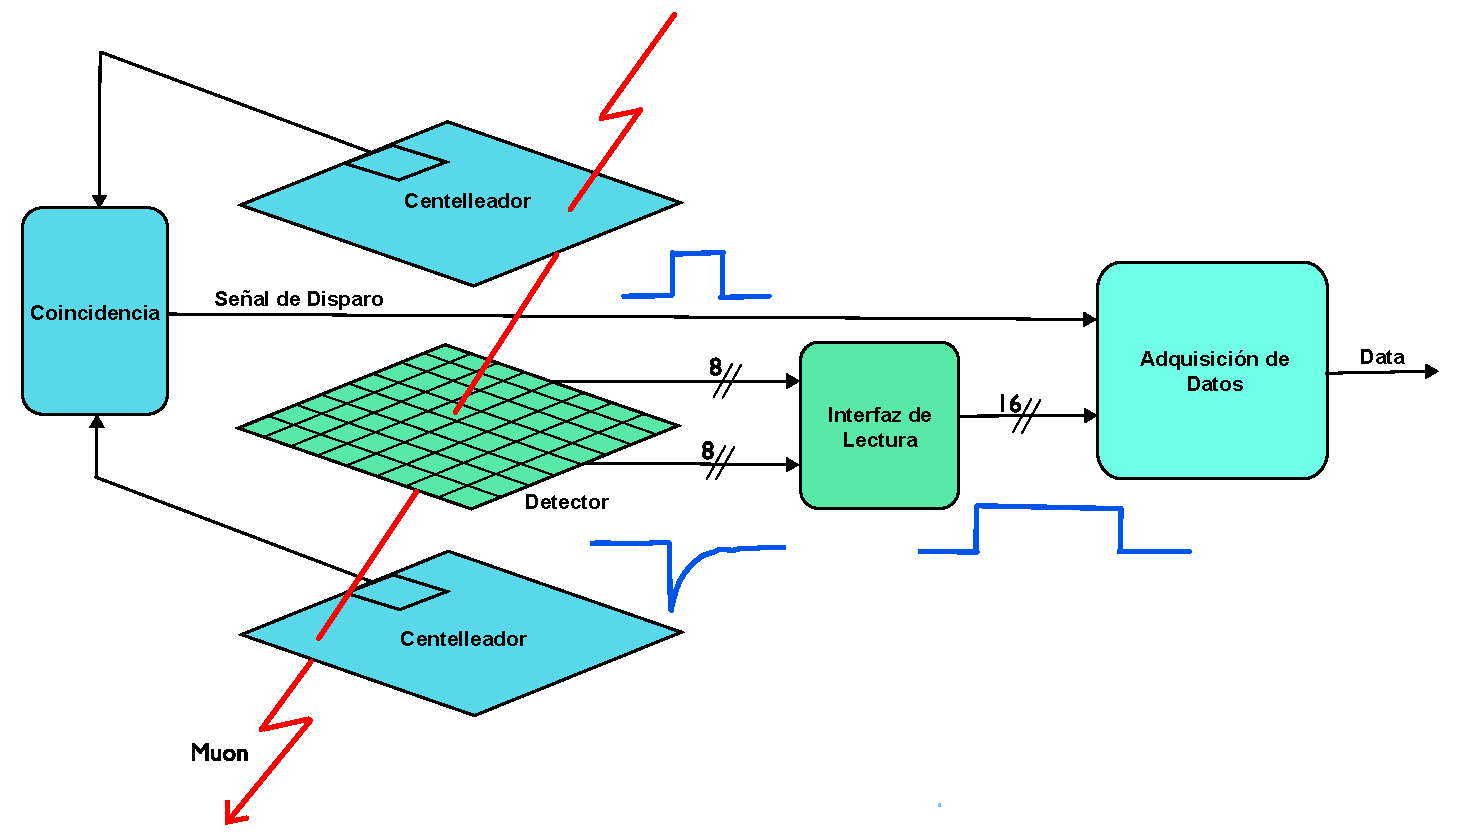
\includegraphics[scale=0.55]{sistema.pdf}
		\caption{Diagrama del sistema de muongrafía de terreno para un solo detector. Se incluyen en azul las formas de señal asociadas a la señal de disparo, eventos de detección, y lectura de pulsos.}
		\label{img:sistema}
	\end{figure}						

\section{Alcances y contribuciones}

\gcnote{Toda esta seccion debe ser mas concreta y especifica.}
	Se espera que este sistema sea capaz de generar información suficiente para representar la ubicación del paso de las partículas en la superficie del detector, determinando cuadrantes de $1cm^2$ que hayan sido excitados por el cruce de partículas.
	
	El sistema deberá ser capaz de captar cantidades pares arbitrarias de canales, discriminando partículas mediante la utilización de las señales de disparo disponibles.
	
	La información generada pasará a etapas siguientes de análisis detallado o de representación gráfica, por lo cual es importante que el sistema sea capaz de entregar información pertinentemente ordenada, procesada y seleccionada para dichos fines.
	
	Finalmente, uno de los principales aportes recae en la documentación respecto a entorno, operación y desarrollo del sistema en cuestión. Esto con el fin de facilitar la implementación del diseño en nuevos sistemas, permitir profundizar y mejorar la propuesta diseñada y entregar las herramientas al centro y a futuros estudiantes para operar dispositivos que posean etapas equivalentes.


\section{Organización del documento.}

	Este documento se estructura de la siguiente manera: \gcnote{demasiados capitulos. No deberian ser mas de 5 o 6.}
	
	\begin{itemize}
		\item El \textbf{Capítulo \ref{cap:art}} incluye el estado del arte en cuanto a dispositivos de adquisición de datos para partículas de altas energías.
		\item El \textbf{Capítulo \ref{cap:arq}} detalla la arquitectura propuesta para la realización de este proyecto, contemplando componentes y estructura del mismo.
		\item El \textbf{Capítulo \ref{cap:stgc}} describe las características del detector de partículas utilizado.
		\item El \textbf{Capítulo \ref{cap:asd}} resume las especificaciones del sistema de lectura para señales provenientes del detector, además de explicar su estructura y funcionamiento.
		\item El \textbf{Capítulo \ref{cap:sampling}} detalla la primera etapa de diseño de hardware, encargada de tomar muestras de los pulsos digitales provenientes de la etapa inmediatamente anterior.
		\item El \textbf{Capitulo \ref{cap:discriminator}} trata sobre el diseño para la etapa de discriminación del sistema de adquisición, la cual selecciona aquellos eventos temporalmente coincidentes con una señal de disparo.
		\item El \textbf{Capítulo \ref{cap:structure}} describe la etapa de estructuración de eventos y su diseño, en donde la información de pulsos capturados es asociada los canales y cuadrantes correspondientes.
		\item El \textbf{Capítulo \ref{cap:analysis}} detalla la etapa de análisis de datos para determinación del paso de partículas cargadas por el detector.
		\item El \textbf{Capítulo \ref{cap:sync}} trata sobre la etapa de sincronización y su diseño, en donde se coordinan eventos capturados por distintos detectores simultáneamente.
		\item El \textbf{Capítulo \ref{cap:comm}} se refiere a la etapa de comunicación serial, a través de la cual el sistema se comunica con computadores externos para envío de datos.
		\item El \textbf{Capítulo \ref{cap:test}} incluye pruebas realizadas en el sistema con el fin de comprobar funcionamiento y resultados del dispositivo.
		\item El \textbf{Capítulo \ref{cap:insights}} resume los resultados de experimentación y desempeño del sistema diseñado.
		\item El \textbf{Capítulo \ref{cap:conclusiones}} incluye las conclusiones finales y trabajo futuro propuesto a partir de lo realizado en este proyecto de titulación.
	\end{itemize}



\newpage
\thispagestyle{empty}
\cleardoublepage

\chapter{estado del arte}
\label{cap:art}
%Estado del arte y arquitectura propuesta
Previo al diseño de este sistema \gcnote{Cual sistema?  Ya cambiaste de seccion (dangling modifier).}, es pertinente conocer el estado del arte de otros sistemas de adquisición de datos para física de partículas, con el fin de contrastar y rescatar las diferentes estrategias y tecnologías empleadas en la actualidad.

Como referencia para el diseño del sistema de adquisición, se han investigado detectores como los descritos en \cite{Basiladze2017Methods1} y \cite{Basiladze2017Methods2}, enfocados a detección de partículas en diferentes rubros y condiciones. En este capítulo se mencionan \gcnote{solo se mencionan o se describen?} tres sistemas relacionados a esta temática, destacando ideas sobre el esquema general de adquisición de datos, tecnologías que se utilizan actualmente para construirlos y  métodos para adquirir y procesar las señales captadas.

\section{LabPet II}
	Dentro de la variedad de detectores estudiados, LabPet II de Larissa Njejimana \gcnote{no es necesario poner al autor.} \cite{Njejimana2013DesignImaging} presenta una estructura clara \gcnote{ que es na estructura clara?} e interesante. Este detector posee un DAQ (Data Acquisition system) distribuido en tres FPGAs, contando con etapas para recolectar, procesar y transmitir la información obtenida. Una primera etapa consiste en registrar tiempo, energía y posición de las partículas captadas; una segunda etapa ordena cronológicamente los eventos capturados, mientras que una tercera etapa agrupa detecciones coincidentes, calculando además la tasa de eventos aleatorios ocurridos. \gcnote{es una FPGA por etapa?}
	
	La Figura \ref{fig:njejimana} ilustra este sistema \gcnote{dangling modifier. Estas cometiendo los mismos errores que antes.}. Se \gcnote{otro mas} compone de 3 FPGAs: una encargada de capturar las señales provenientes de los detectores, llamada \textit{Front-End board}; otra dedicada a ordenar los eventos y corregir datos, llamada \textit{Hub board}; y una última FPGA encargada de seleccionar eventos válidos y coincidentes, llamada \textit{Coincidence board}, la cual puede conectarse a múltiples Hub boards. \gcnote{Suena redundante con el parrafo anterior. Juntar y uniformar ambos parrafos.} Los resultados son enviados a un computador, el cual también permite configurar y ajustar parámetros en las Hub y Coincidence boards.
	
	Si bien los detectores de LabPet II están diseñados para otro tipo de partículas (positrones), la naturaleza de las señales es muy similar a los muones, y por lo tanto la lógica para su adquisición y procesamiento es comparable. Aún así, la cantidad de señales que es capaz de manejar dicho dispositivo ronda las 64 señales por módulo, a tasas cercanas a los 2 millones de eventos por segundo, las que comparativamente sobrepasarían las necesidades del sistema a desarrollar en este proyecto de titulación. Por ejemplo, los rayos cósmicos cruzan el planeta tierra a aproximadamente 1 rayo cósmico por minuto en un área de $1cm^2$, muy por debajo de lo que se espera en LabPET II. \gcnote{SI bien es mas de lo que se necesita, deberia funcionar para la aplicacion.  Por que hacer otro y no solo replicar este?}
	
	Del sistema de adquisición para el detector anteriormente mencionado, se destaca la utilización de multiplexores, serializadores/deserializadores y memorias de almacenamiento temporal (\textit{buffer}). Dada la naturaleza y cantidad de eventos, se hace necesario serializar la información, ya que de otro modo sería necesario construir dispositivos con múltiples puertos de entrada o incluir varios del mismo tipo. Además, debido a la frecuencia de los eventos, se hace obligatoria la existencia de \textit{buffers} para el almacenamiento de la información, permitiendo procesarlos y transmitirlos hacia etapas posteriores a tasas menores. Es destacable también la utilización de métodos para ordenar cronológicamente los eventos y la implementación del método TOT (Time-over-threshold) \gcnote{referencia?} para el calculo de energía y datos temporales de pulsos analógicos. Este último es el método utilizado por la interfaz de lectura presente en el proyecto sTGC Minería.
	
	\begin{figure}[h]
		\centering
		\includegraphics[scale=0.45]{njejimana.png}
		\caption{Diagrama de bloques del sistema de adquisición de datos para LabPET II \cite{Njejimana2013DesignImaging}}
		\label{fig:njejimana}
	\end{figure}
	
\newpage
\section{4D PET}
	Otro sistema de referencia es el DAQ para el sistema modular 4D PET \cite{Marcatili2011DevelopmentDetector}. Este dispositivo permite capturar gran cantidad de señales \gcnote{Cuantas? Orden de numeros?} provenientes de arreglos matriciales de fotomultiplicadores. Se caracteriza principalmente por poseer una tarjeta madre central, en la cual es posible conectar hasta 18 tarjetas de adquisición. Cada una de estas tarjetas tiene de 8 a 32 canales para adquisición de señales, y su función es capturar, procesar y enviar información a la placa madre. La Figura \ref{fig:marcatili} ilustra la arquitectura de este sistema.
		
	Las señales son capturadas por ASICs (\textit{Application Specific Integrated Circuits}), muestreadas por conversores análogo-digitales y procesadas por una FPGA, mientras que una FPGA principal (etiquetada como Master FPGA) se encarga de controlar a las FPGAs anteriores y de recibir los datos capturados. El procesamiento inicial de las señales se encarga de calcular energía y datos temporales asociados a las partítuclas detectadas, mientras que el procesamiento final relaciona los eventos que hayan sido temporalmente coincidentes enter sí y a su vez calcula el tiempo de vuelvo de las partículas, mediante un conversor de tiempo a señal digital (TDC).
	       	
	Este sistema destaca por su modularidad, la cual permite un fácil escalamiento. En contraste con LabPET II, se utilizan varias placas adquisidoras paralelas en vez de utilizar serialización de datos, permitiendo procesar la información antes de llegar a la FPGA principal. Cabe destacar que esta arquitectura está relacionada con la necesidad de encontrar múltiples eventos simultáneos en distintas ubicaciones, requerimiento que no está presente en el sistema que se planea diseñar para este proyecto de titulación. 
	
	\begin{figure}[h]
		\centering
		\includegraphics[scale=0.4]{marcatili.png}
		\caption{Diagrama de bloques del sistema de adquisición de datos para Detector PET 4D \cite{Marcatili2011DevelopmentDetector}}
		\label{fig:marcatili}
	\end{figure}
	
\newpage
\section{ATLAS}
	Finalmente, la referencia más importante corresponde al experimento ATLAS \cite{Spieler2012ElectronicsAcquisition}, ya que una de sus etapas utiliza detectores sTGC, mientras que otra de sus etapas utiliza la misma interfaz de adquisición que será utilizada en sTGC Minería.

	El experimento ATLAS se encarga de interceptar grupos de partículas provenientes de haces de protones acelerados en el LHC (Large Hadron Collider) en CERN, con el objetivo de estudiar las colisiones de partículas ocurridas a su paso. Las colisiones se generan aproximadamente cada $25\mu$s\cite{Whiteson2016TheSystem}, y cada colisión pruduce cerca de 23 interacciones con el detector, que junto a otros factores implica cerca de $10^9$ eventos cada segundo. La tasa de aparición y nivel de energía de estos eventos son las principales razones por las que este detector es tecnológicamente complejo.
	
	El estudio de colisiones tiene como objetivo medir partículas conocidas y deducir la existencia de partículas nuevas. Para lograrlo, es necesario reconstruir las trayectorias e interacciones de todas las partículas medibles mediante múltiples y variados sistemas de detección. Uno de estos sistemas corresponde al Espectrómetro de Muones, \gcnote{referencia?} el cual permite determinar la validez de los eventos y trazar la trayectoria de los muones emitidos en las colisiones. 
	
	El Espectrómetro de Muones se compone de 4 tecnologías de detección diferentes, una de las cuales corresponde a los detectores sTGC ubicados en la ya mencionada Small Wheel \gcnote{haz una referencia a donde se hizo la mencion. El lector ya se olvido a esta altura.}. Otra de las tecnologías de detección que componen al Espectrómetro corresponde a los detectores TGC (Thin Gap Chamber), los cuales se diferencian de los detectores sTGC en el tamaño de sus componentes. Los detectores TGC están ubicados en el sector denominado Big Wheel, indicado en la Figura \ref{fig:both-wheels}, y sus datos son obtenidos gracias a una interfaz de lectura llamada ASD (Amplificator-Shaper-Discriminator). Esta inferfaz de lectura, en conjunto con detectores sTGC, da vida al proyecto sTGC Minería en CCTVal, y su funcionamiento será explicado con mayor detalle en el Capítulo \ref{cap:sdet}.
	
	\begin{figure}[h]
		\centering
		\includegraphics[scale=0.5]{atlas-layout-big-small-wheel.png} 
		\caption{Layout del experimento ATLAS, donde se indica la posiciónde la Small Wheel y la Big Wheel\cite{Formenti2018CERNReport}}
		\label{fig:both-wheels}
	\end{figure}
	
	La Figura \ref{fig:spieler} ilustra el sistema de captura de datos para detectores TGC del Big Wheel en el Espectrómetro de Muones. Los muones son representados con el símbolo $\mu$ y cruzan tres capas de detectores TGC, cada una de las cuales cuenta con sus interfaces de lectura ASD. Los bloques posteriores se encargan de pre-procesar los pulsos capturados y entregarlos a las posteriores etapas de lectura y de selección de eventos.
	
	\begin{figure}[h]
		\centering
		\includegraphics[scale=0.6]{spieler.png}
		\caption{Diagrama de la interfaz de captura para detectores de muones TGC \cite{Spieler2012ElectronicsAcquisition}. Los muones se representan con el símbolo $\mu$. Existen 3 capas de detectores, por lo tanto se observan 3 bloques que incluyen retardos, selección y captura de los pulsos.}
		\label{fig:spieler}
	\end{figure}

	En ATLAS, la selección de eventos a ser estudiados se lleva a cabo en dos etapas. La primera de ellas, llamada \textit{Level 1 Trigger}, involucra al Espectrómetro de Muones y calorímetros. La segunda etapa involucra algoritmos distribuidos en varios computadores y se le conoce como \textit{High-level Trigger}. La Figura \ref{fig:colombo} ilustra ambas etapas en paralelo a los sistemas de lectura de datos. El sistema de lectura de datos ilustrado en \ref{fig:spieler} corresponde al cuadro amarillo ubicado en la esquina superior derecha de la Figura \ref{fig:colombo}, etiquetado como \textit{Muon}. Si el Level 1 Trigger aprueba un evento detectado por el Espectrómetro y los calorímetros, entonces inicia la adquisición de estos datos en la tarjeta de lectura (etiquetada como \textit{Readout System} en la Figura \ref{fig:colombo}). Además, el Level 1 Trigger envía información sobre regiones de interés a analizar, con el fin de llevar a cabo la segunda etapa de selección (\textit{High-Level Trigger}). Esta segunda etapa de selección utiliza software distribuido en cerca de 2000 computadores conectados a una red Ethernet y filtra eventos en función a muestras de datos pertenecientes a las regiones de interés calculadas por el Level 1 Trigger\cite{Colombo2015Data-flowCase}. Finalmente, los eventos seleccionados son trasferidos y  almacenados en los bancos de datos del centro de investigación.
	
	\begin{figure}[h]
		\centering
		\includegraphics[scale=0.56]{colombo.png}
		\caption{Diagrama del sistema de disparo y adquisición de datos en el experimento ATLAS. \cite{Colombo2015Data-flowCase}}
		\label{fig:colombo}
	\end{figure}
	
	Entrando aún más en detalle, el verdadero sistema de adquisición de datos para este experimento es el software distribuido en red\cite{Whiteson2016TheSystem}, capaz de discriminar, procesar y transferir los eventos seleccionados a los bancos de datos. El sistema lectura (\textit{Readout System}) en conjunto con el disparo de primer nivel solo serían un equivalente a una interfaz de captura muy sofisticada, pero para el caso de esta memoria de titulación este sistema sería comparable al sistema de adquisición que se desea diseñar. \gcnote{No se entiende que quieres decir aca. Reescribir.}
	
	El Readout System consiste en una tarjeta llamada ROBIN, compuesta de buffers, chips de comunicación, memoria flash, procesador y una FPGA, como se ilustra en la Figura \ref{fig:whiteson}
	
	\begin{figure}[h]
		\centering
		\includegraphics[scale=0.7]{whiteson.png}
		\caption{Diagrama de la tarjeta de lectura ROBIN en ATLAS \cite{Whiteson2016TheSystem}.}
		\label{fig:whiteson}
	\end{figure}
	
	La lógica implementada en la FPGA se ilustra en la Figura \ref{fig:whiteson2}. Se observa que su labor es principalmente controlar los buffers de datos, traspasar los eventos captados hacia la siguiente etapa y eliminar los datos descartados por la señal de disparo de alto nivel.
	
	\begin{figure}[h]
		\centering
		\includegraphics[scale=0.7]{whiteson2.png}
		\caption{Diagrama de bloques de la FPGA en ROBIN \cite{Whiteson2016TheSystem}.}
		\label{fig:whiteson2}
	\end{figure}
	
	\newpage
	Si bien este \gcnote{dangling} detector es comparativamente más complejo que los anteriores, presenta elementos comunes es su composición, sobretodo en la utilización de ASICs y FPGA para captura y control de los datos adquiridos. Se asemeja funcionalmente al 4D PET, en el sentido de implementar múltiples instancias de hardware equivalente, para así lograr manejar mayor cantidad de datos y brindar mayor control en cada uno de ellos. El fuerte de este detector radica en su conectividad en red y sistemas distribuidos, necesarios para la gran cantidad de datos simultáneos que deben ser procesados. 


\section{Discusión sobre alternativas existentes}
	Es claro que la tendencia en desarrollo de sistemas de adquisicón es la utilización de ASICs en etapas de primera lectura, mientras que se utilizan FPGAs en etapas de manejo de datos y preprocesamiento, principalmente debido a la magnitud temporal de las señales, a la alta necesidad de precisión en su sincronización, y a la gran cantidad de señales de entrada que deben ser atendidas.
	
	Los elementos más utilizados y recomendados a implementar son los buffers de almacenamiento, principalmente para ajustar la tasa de transmisión de datos de la captura hacia las siguientes etapas de procesamiento, que suelen ser más lentas. En el sistema que se planea diseñar esto no es un problema, ya que la tasa de eventos es muy baja en comparación a los detectores estudiados. Aún así, pueden ser útiles \gcnote{que cosa puede ser util?} para el escalamiento de los detectores en el futuro.
	
	El concepto de serialización de datos estuvo principalmente presente en el detector LabPET II. Es pertinente considerarlo, sobretodo para el escalamiento del detector de muones. En caso de requerir cubrir un área mayor o con varias capas superpuestas de detectores, será necesario captar mayor cantidad de señales. Es allí donde se debe decidir si es recomendable comenzar con serialización de datos o con paralelismo de hardware.% Además, dado que es necesario tener noción del tiempo de ocurrencia de los eventos, podría asociarse este dato a cada pulso, facilitando la implementación de serialización de datos. Esto no sería una desventaja, ya que no existe real necesidad de procesar datos de manera rápida y simultanea, reduciendo costos en hardware, pero aumentando esfuerzos de ingeniería.
	
	%Para el caso de pre-procesamiento, selección, formateo y transmisión de datos se puede considerar agregar procesadores dedicados en conjunto con la FPGA principal, que si bien no fueron encontrados textualmente en los ejemplos indicados, sí pueden ser de utilidad, sobretodo dada la existencias de chips que incluyen FPGA en conjunto con procesadores, como los SoC (\textit{System on Chip}) Zynq.
	
	% Finalmente, puede ser interesante incluir métodos de TDC para conversión de la señal digital generada por la placa acondicionadora ASD. La duración de esta señal tiene relación con la amplitud y la energía de los pulsos analógicos captados, lo que podría ser muestreado con una implementación similar a la indicada en \cite{Arpin2010AResources}.
	
	En resumen, es conveniente diseñar el sistema en una FPGA dedicada a la adquisición de datos, incluyendo buffers de almacenamiento para los eventos capturados y replicando este sistema para cada detector adicional.
	

\newpage
\thispagestyle{empty}
\cleardoublepage

\chapter{sistema de detección}
\label{cap:sdet}
El proyecto sTGC Minería se compone de tres sistemas principales: disparo, detección y adquisición, como se ilustra en la Figura \ref{fig:sistema-completo}. Como se introdujo en la Sección \ref{sec:planteamiento}, el sistema de disparo \cite{Oyanadel2020SistemaSTGC} (ilustrado en azul),  está formado por dos detectores centelladores y una unidad de coincidencias que emite una señal digital de disparo (indicada en celeste) cuando un muon traspasa ambos detectores centelladores. Esta señal de disparo es necesaria para discriminar eventos captados por el detector sTGC y descartar interacciones procedentes de otras partículas cargadas que no sean muones. \gcnote{(Para discutir) Este sistema de deteccion ya se encuentra fabricado? Por que no se trata en este trabajo?}
	
Si bien los detectores centelladores presentes en el sistema de disparo son capaces de detectar exclusivamente el paso de muones, estos no son capaces de determinar la ubicación del vértice de interacción. Para cumplir con este requerimiento de localización, se utilizan los detectores complementarios al sistema de detección sTGC (ilustrados en verde en la Figura \ref{fig:sistema-completo}) \gcnote{revisar colores}, sistema que es capaz de determinar la ubicación de los vértices de interacción gracias a su tecnología de fabricación.
	
En este capítulo se detalla la forma y funcionamiento del sistema de detección, describiendo el prototipo de detector sTGC utilizado en sTGC Minería y describiendo también la interfaz de lectura ASD \gcnote{introdujiste ASD?} que lo sucede. \gcnote{Clarificar explicitamente si esto ya esta implementado o haras algo con esto en tu memoria.}Es necesario conocer las características de estas etapas, ya que determinan la cantidad y tipos de señales a leer en el sistema de adquisición de datos a ser diseñado en este proyecto de titulación.
	

\gcnote{Estudiar este sistema fue parte de tu memoria?}

	\begin{figure}[h]
		\centering
		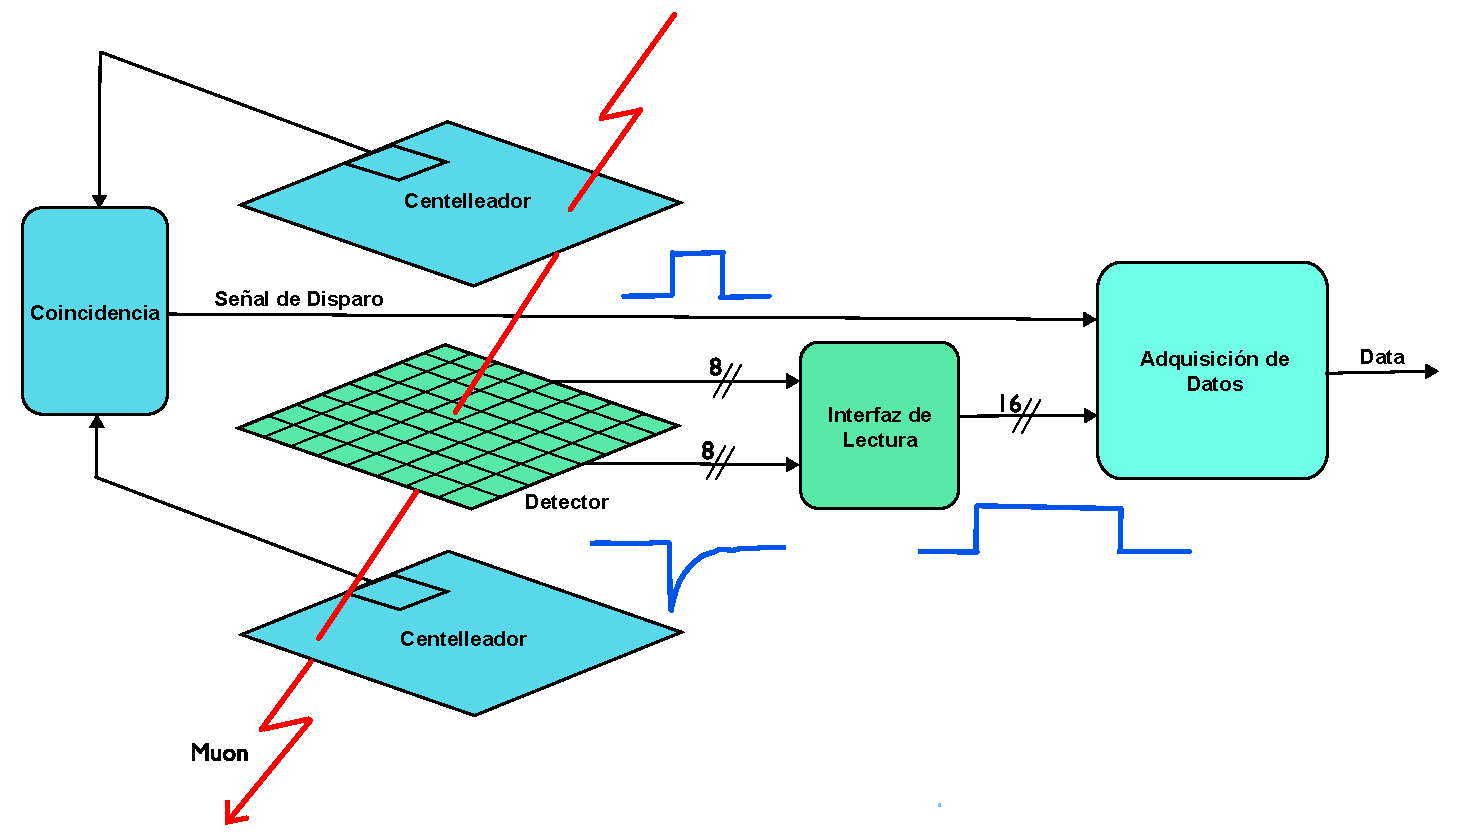
\includegraphics[scale=0.55]{sistema.pdf}
		\caption{Diagrama del sistema de muongrafía de terreno utilizando un solo detector.}
		\label{fig:sistema-completo}
	\end{figure}

	\section{Detector de Partículas}
	\label{sec:stgc}
	
La detección de muones en este proyecto es realizada mediante un detector de partículas inspirado en los detectores sTGC del experimento ATLAS, como se mencionó en la Sección \ref{par:smallwheel}. Los detectores originales se ubican en la llamada Small Wheel de ATLAS, formando parte del Espectrómetro de Muones, el cual se encarga de determinar el momento y la trayectoria de los muones emitidos por las colisiones. Para el proyecto sTGC minería, CCTVal construyó un prototipo de detector sTGC a menor escala utilizando la misma tecnología de fabricación presente en los detectores originales. En esta sección se describe la estructura de un sTGC original y la del prototipo en cuestión, incluyendo información sobre el funcionamiento y operación del prototipo de detector sTGC fabricado en CCTVal.

\begin{figure}[h]
	\centering
	\includegraphics[scale=0.7]{tgc-structure.png}
	\caption{Estructura interna de un detector sTGC\cite{Chapman2014ATLASUpgrade}.}
	\label{img:stgc-structure}
\end{figure}

\subsection{Estructura general} 
	Un sTGC está compuesto por dos planos de grafito (cátodos), con múltiples cables en medio (ánodos)\cite{Formenti2018CERNReport}, tal como se observa en la Figura \ref{img:stgc-structure}. Recubriendo el exterior de ambos cátodos se ubican capas aislantes que separan los cátodos de las zonas conductoras, llamadas ``\textit{pads}'' en la cara superior y ``\textit{strips}'' en la cara inferior del detector, diferenciándose en la forma y área que abarca cada uno. Los \textit{strips} corresponden a delgados rectángulos de cobre, mientras que los \textit{pads} son mantos de cobre más anchos, equivalentes al área de varios \textit{strips}. Los cables al interior del detector se encuentran orientados perpendicularmente respecto a los \textit{strips} y en paralelo a los \textit{pads}.
	
	\newpage
	Al interior del detector, entre los planos de grafito, se infiltra un gas compuesto por dióxido de carbono y n-pentano\cite{Formenti2018CERNReport}. Mediante la aplicación de alto voltaje se genera un campo eléctrico entre ánodos y cátodos. Se utilizan 3000 V$_{DC}$ entre cátodos y ánodos para generar el campo eléctrico, limitando la corriente a 50uA. El gas en el interior puede ser dióxido de carbono puro, pero esto genera mayor probabilidad de generar descargas no asociadas a muones. La Figura \ref{img:stgc-field} representa un corte transversal de un detector y sus líneas de campo eléctrico desde ánodo (cables) hasta cátodos (lámina de grafito superior e inferior). 
	
	El paso de muones a través del detector genera la ionización del gas y la liberación de electrones, los cuales son captados por los cables del detector gracias al campo eléctrico. El flujo de electrones en el gas ionizado genera pulsos de corriente en los cables, produciendo diferencia de potencial en los cátodos. Esta diferencia de potencial interactúa con los \textit{pads} y \textit{strips} en el exterior del detector, generando pulsos de voltaje en estas zonas conductoras, pero con polaridad inversa respecto a la corriente presente en los cables. En la Figura \ref{fig:sistema-completo}, el pulso de voltaje correspondiente a la señal de salida de un canal de detección está representado por el pulso verde dibujado en la zona central de la imagen.
	
	La amplitud de los pulsos generados en el detector será mayor en torno al vértice de interacción y menor en zonas lejos de él. Esto permite relacionar la posición y energía de la partícula con las amplitudes de los pulsos en cada \textit{strip} o cable medido.
	
	\begin{figure}[h]
		\centering
		\includegraphics[scale=0.3]{stgc-transversal.png}
		\caption{Líneas de campo eléctrico observadas en un corte transversal de los cables y cátodos del detector. Los cátodos se ilustran en celeste, los cables se representan como puntos negros, y las lineas de campo corresponden a las flechas de color rojo\cite{DeSmet2011StudyLab}.}
		\label{img:stgc-field}
	\end{figure}

\subsection{Detector sTGC utilizado}
	En ATLAS, los vértices de interacción se determinan leyendo las señales provenientes de \textit{strips} y cables al mismo tiempo. Debido a que los \textit{strips} son perpendiculares a los cables, su lectura forma un cuadrante imaginario de dos ejes coordenados (\textit{strips} vs. cables), similar al presentado en la Figura \ref{img:cuadrantes-ministgc}. Por ejemplo, si un muon interactúa con un cable y un \textit{strip} al mismo tiempo, significa que el vértice de interacción se ubica en las cercanías de la intersección \textit{strip}/cable. Sin embargo, para el trabajo considerado en esta memoria de titulación se leerán solo las señales provenientes de \textit{strips}, por los que se estará midiendo un solo eje de posición y será necesario agregar un segundo eje coordenado para poder determinar los vértices de interacción. La ventaja de leer señales desde \textit{strips} es que las señales medibles en ellos son de fácil acceso, debido a que los \textit{strips} son superficies conductoras expuestas al exterior y permiten incorporar conectores sobre ellos sin mayor dificultad.
	
	Para agregar un eje coordenado adicional al detector, se reemplazan los \textit{pads} de la cara superior por \textit{strips} perpendiculares a los del plano contrario. Así se logra tener información bidimensional del paso de una partícula leyendo solo las señales provenientes de \textit{strips} perpendiculares entre sí. La Figura \ref{img:stgc-mini-estructura} ilustra la composición del detector capa por capa y detalla la orientación de cables y \textit{strips}.
	
	\begin{figure}[h]
		\centering
		\includegraphics[scale=1]{stgc-mini-estructura}
		\caption{Estructura interna de un detector sTGC adaptado para este proyecto de titulación. El gas es contenido entre ambas capas de grafito (cátodos). Los cables internos corresponden a los ánodos.}
		\label{img:stgc-mini-estructura}
	\end{figure}

	En particular, en cada cara del detector utilizado se cuenta con 8 \textit{strips} de 15cm de largo y 1cm de ancho cada uno, sin contar los \textit{strips} en los bordes del detector debido a que el área abarcada por estos es diferente a la forma de un \textit{strip} estándar, entorpeciendo la medición y posterior reconstrucción de datos. %\sgcnote{hay strips inutiles?}\jgnote{efectivamente}.
Una fotografía de este detector se incluye en la Figura \ref{img:foto-mini-stgc}. En la parte superior de la fotografía, en recuadros verdes, se observan tubos para el flujo de gas. Por abajo, en amarillo, se indican 8 cables coaxiales conectados a los \textit{strips} de la cara superior del detector. A la izquierda están situados los otros 8 cables correspondientes a los \textit{strips} de la cara inferior, también etiquetados en amarillo. En el costado derecho, en el recuadro azul, existe una red resistiva para la lectura de cables internos del detector, los cuales no serán utilizados en este proyecto. % \sgcnote{marcar claramente estas componentes en la figura.}.
	
	\begin{figure}[h]
		\centering
		\includegraphics[scale=0.08]{mini-stgc2.jpg}
		\caption{Vista superior del detector prototipo.}
		\label{img:foto-mini-stgc}
	\end{figure}	
	
	Dado que los \textit{strips} de la cara superior del detector son perpendiculares a los de la cara inferior, es posible interpretar el detector como un cuadrante de ejes coordenados según se ilustra en la Figura \ref{img:cuadrantes-ministgc}. En esta figura, cada cuadro representa un área de detección de 1cm$^2$, la cual corresponde a la precisión para la determinación de los vértices de interacción. Como el detector posee 8 \textit{strips} por cara, se tiene un total de 16 canales de detección, los que en su conjunto forman 64 zonas de detección de 1cm$^2$. Los \textit{strips} de la cara superior se nombrarán como el eje X, mientras que los \textit{strips} correspondientes a la cara inferior del detector serán asociados al eje Y, siendo el cuadro (0,0) aquel que se ubica en la zona de detección inferior izquierda.
	
	\begin{figure}[h]
		\centering
		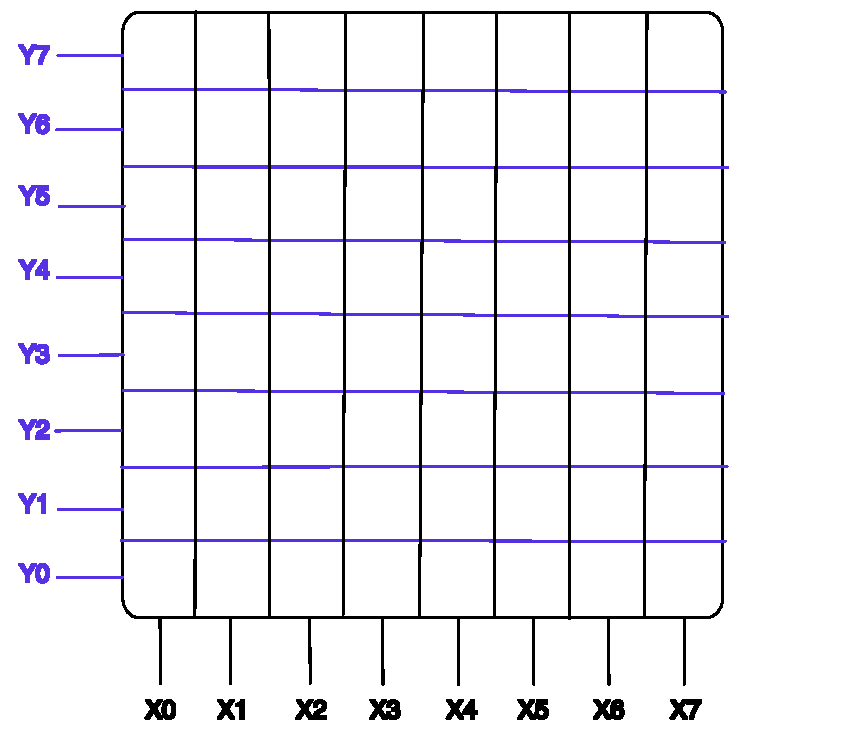
\includegraphics[scale=0.55]{cuadrantes-ministgc.pdf}
		\caption{Vista superior del detector, en donde se indican las etiquetas asociadas a cada canal en función del eje al que pertenece. Cada cuadro representa un área de detección de 1cm$^2$.}
		\label{img:cuadrantes-ministgc}
	\end{figure}

\subsection{Procedimiento de operación y pruebas}
	Antes de poner en marcha mediciones o experimentos con un nuevo detector, se deben realizar ajustes, caracterizaciones y pruebas que permitan corroborar el correcto funcionamiento del dispositivo. Para esto, se recomienda llevar a cabo una secuencia de experimentos con el fin de comprobar el funcionamiento de cada canal y medir el ruido base, la frecuencia de detección y las amplitudes medias esperadas.

	\subsubsection{Dispositivos para lectura de señales}
		Para observar los pulsos captados por el detector es necesario contar con un sistema de lectura adecuado. Este dispositivo deberá poseer una  baja impedancia, menor a 100$\Omega$ para evitar atenuaciones y reflexiones, así como también deberá contar con una etapa de amplificación tal que permita medir sin problemas las señales captadas con un osciloscopio, digitalizador o un sistema para adquisición de datos. Las señales emitidas por el detector rondan el orden de los milivolts, lo cual significa que el sistema de lectura debe poseer una ganancia tal que la magnitud de la señal de salida esté dentro de la resolución de voltaje del aparato de medición.
		
		Un ejemplo de sistema de lectura es la interfaz ASD mencionada en la Sección \ref{sec:atlas}, la cual será utilizada en este proyecto de titulación. Esta interfaz está diseñada para la correcta lectura de \textit{strips} y cables provenientes de detectores TGC, contando con una amplificación inicial de 0.8V/pC de carga y con una segunda etapa capaz de amplificar 7 veces la señal entrante. Además, la primera etapa de amplificación de la interfaz ASD se encarga de darle forma al pulso captado, con el fin extender la señal en el tiempo y facilitar su muestreo.
		
		%La interfaz ASD cuenta con salidas digitales de tipo LVDS. Estas señales representan el tiempo que la señal permanece por sobre un umbral arbitrario configurado, el cual será proporcional a la amplitud y por tanto a la carga del pulso medido. Cuenta también con una única señal análoga conectada al canal 16 (\textit{Hit} 15), proveniente de la pre-amplificación. Esta es una señal de monitoreo ideal para realizar pruebas de funcionamiento.
		

	\subsubsection{Estimación de ruido base}
		Una vez escogidos los métodos de lectura y las herramientas de muestreo a utilizar, es necesario medir el ruido base del detector. Este ruido corresponde a distorsiones propias del dispositivo, como fugas de corriente, conducción indeseada y ruido electromagnético. Conocer el ruido base permite filtrar el ruido para el análisis de eventos de interés.
		
		Para realizar la medición de ruido base en este detector prototipo se debe hacer circular el dióxido de carbono (o mezcla de dióxido de carbono y N-Pentano). Antes de proceder a realizar mediciones, es necesario esperar a que el detector haya sido llenado totalmente de gas. Dada su área interior cercana a los 225cm$^2$, el detector se encontrará completamente infiltrado con gas tras 20 minutos de operación. %\sgcnote{Especificar que estos son pasos y procedimientos para el detector en particular.  Como estan, suenan muy absolutos, como que siempre se deb hacer asi y no hay otra forma.}
		
		Cuando el detector se encuentra totalmente lleno de gas, se procede a medir el ruido base en cada uno de sus canales, sin conectar el detector a su fuente de alto voltaje. Estas mediciones permiten generar histogramas de ruido, los cuales han de tener una distribución gaussiana en condiciones normales de operación\cite{Naseri2021ATLASILC}. %\sgcnote{Puedes mostrar resultados de esto?}\sjgnote{lamentablemente no tengo datos para mostrar, es parte de las pruebas de caracterizacion del detector que se deben realizar de manera presencial de un laboratorio, pero encontre una referencia del proyecto ATLAS donde se observa ruido base en un histograma junto a otros datos sin indicar su distribucion de manera explicita. Servira?}
		
		La amplitud del ruido base definirá una zona que deberá ser considerada en los análisis de eventos. Pulsos dentro de este rango de amplitudes no serán correctamente captados. Por otro lado, se espera que el ruido sea menor que la amplitud media de los eventos generados por cruce de muones en el detector.
		
		Conocer tanto la amplitud del ruido base como la de los pulsos originados por muones, permite escoger señales de disparo en la tarjeta ASD, o filtros digitales en las etapas de análisis. 
		
	\subsubsection{Observación de falsas detecciones}
		Para una fiel interpretación de la información captada por un detector, es importante conocer la distribución y frecuencia de detecciones que no correspondan a cruce de muones. La medición de estos parámetros requiere la generación del campo eléctrico dentro del detector conectando su respectiva fuente de alto voltaje.
		
		Una vez generado el campo eléctrico, es posible captar falsas detecciones o disparos aleatorios producto de la conductividad de los materiales o fugas de corriente. Estos eventos suelen tener una distribución normal y ser de amplitudes mayores a la de interés (muones). Conocer esta información permite ignorar señales sobre un umbral tal que se correspondan con amplitudes de eventos no deseados.
	
	\subsubsection{Detección de partículas}
		Para comprobar el correcto funcionamiento del detector, es de gran utilidad utilizar fuentes radioactivas para generar pulsos de prueba. Aunque una fuente radioactiva de rayos Gamma genera pulsos de mayor amplitud que eventos producidos por muones, esta permite comprobar la correcta operación de cada canal y la distribución de carga del evento en cada canal adyacente.
	
		Para el caso de detección de muones, es importante contar con un sistema de disparo para ignorar detecciones provenientes de otras partículas cargadas capaces de ionizar el gas al interior del detector. Para el caso de sTGC, se cuenta con el sistema de detectores centelladores mencionados con anterioridad e ilustrados en la Figura \ref{fig:sistema-completo}. Se recomienda posicionar uno de estos detectores sobre el detector sTGC, cubriendo un área igual a la que abarque el sTGC. De ser factible, se recomienda incluir un segundo detector centellador por debajo, para generar una señal de disparo conjunta con el centellador superior. Esto permite descartar incidencias casi horizontales de muones, pasando por un centellador pero no por el detector sTGC.
		
	
	\section{Interfaz de Lectura}
	\label{sec:asd}
	La interfaz de lectura ASD (Amplificator-Shaper-Discriminator)\cite{1999ATLASICs} es un sistema de 16 canales utilizado para la lectura de detectores TGC en la Big Wheel del experimento ATLAS, como se mencionó en la Sección \ref{sec:atlas}. El propósito principal de esta interfaz es detectar pulsos de alta frecuencia provenientes de detectores TGC, los cuales forman parte del Level-1 Trigger en el Espectrómetro de muones. Cada canal se corresponde con un \textit{strip} o cable de un detector, por lo que al analizar las señales de salida de esta tarjeta permite determinar los vértices de interacción \sgcnote{Revisa la gramatica, en particular tildes. Ya he corregido varios directamente en el texto, pero ya parece algo sistemativo y no puedo estar corrigiendo uno por uno.} de muones con el detector.

La Figura \ref{img:asd-board} corresponde a una fotografía de esta interfaz, destacando sus conectores principales y sus canales de entrada. Los canales son llamados \textit{Hits} y se enumeran del 0 al 15. La interfaz ASD posee \sgcnote{dangling. Quien posee?  Ultimo que corrige, ya hemos discutido como 100 veces esto} un conector de 40 pines para la conexión de su fuente de voltaje, transmisión de las señales de salida  e ingreso de pulsos de prueba \sgcnote{Revisar esto, demasiados para, para, para...}. El detalle de cada pin se ilustra en la Tabla \ref{tab:asd-ports}, donde las columnas izquierdas corresponden a los terminales positivos de los pares diferenciales, mientras que las columnas derechas indican los terminales negativos.  \sgcnote{y el punto? Mejorar la resolucion de la figura. Es una tabla. Seria mejor hacerla directo en latex.  En general, se nota que aca escribiste a la rapida sin revisar, y se nota una diferencia entre este texto y el resto (como pegado con chicle.  Debes evitar que eso se refleje en el documento.}

\begin{figure}[h]
	\centering
	\includegraphics[scale=0.55]{asd-board.png}
	\caption{Interfaz de lectura ASD. Se destacan en la imagen sus canales (hit) del 0 al 15, su salida analógica LEMO y el primer pin en su conector de 40 posiciones.}
	\label{img:asd-board}
\end{figure}

% Please add the following required packages to your document preamble:
% \usepackage{booktabs}
\begin{table}[]
	\centering
	\begin{tabular}{@{}llll@{}}
		\toprule
		\textbf{Pin} & \textbf{Nombre} & \textbf{Nombre}                & \textbf{Pin} \\ \midrule
		1            & GND             & V$_{th}$                       & 2            \\
		3            & -3,0V           & GND                            & 4            \\
		5            & +3,0V           & +3,0V                          & 6            \\
		7            & test pulse      & $\overline{\mbox{test pulse}}$ & 8            \\
		9            & hit 0           & $\overline{\mbox{hit 0}}$      & 10           \\
		11           & hit 1           & $\overline{\mbox{hit 1}}$      & 12           \\
		13           & hit 2           & $\overline{\mbox{hit 2}}$      & 14           \\
		15           & hit 3           & $\overline{\mbox{hit 3}}$      & 16           \\
		17           & hit 4           & $\overline{\mbox{hit 4}}$      & 18           \\
		19           & hit 5           & $\overline{\mbox{hit 5}}$      & 20           \\
		21           & hit 6           & $\overline{\mbox{hit 6}}$      & 22           \\
		23           & hit 7           & $\overline{\mbox{hit 7}}$      & 24           \\
		25           & hit 8           & $\overline{\mbox{hit 8}}$      & 26           \\
		27           & hit 9           & $\overline{\mbox{hit 9}}$      & 28           \\
		29           & hit 10          & $\overline{\mbox{hit 10}}$     & 30           \\
		31           & hit 11          & $\overline{\mbox{hit 11}}$     & 32           \\
		33           & hit 12          & $\overline{\mbox{hit 12}}$     & 34           \\
		35           & hit 13          & $\overline{\mbox{hit 13}}$     & 36           \\
		37           & hit 14          & $\overline{\mbox{hit 14}}$     & 38           \\
		39           & hit 15          & $\overline{\mbox{hit 15}}$     & 40           \\ \bottomrule
	\end{tabular}
	\caption{Detalle de los puertos en el conector de 40 posiciones en la interfaz ASD.}
	\label{tab:asd-ports}
\end{table}

Como su acrónimo lo indica, la interfaz ASD (Amplificator-Shaper-Discriminator) \jgnote{Decidi introducir de nuevo esta sigla, a pesar de que ya la defini anteriormente en el primer párrafo de esta seccion y en la Seccion \ref{sec:atlas}, porque hablo especificamente de su significado} amplifica la carga eléctrica captada desde un canal de un detector, \sgcnote{por que semicolon?} modifica la forma del pulso eléctrico en cuanto a su tiempo de duración y a su amplitud de corriente con el fin de simplificar su posterior medición, y discrimina la amplitud del pulso mediante un circuito comparador. Esta comparación se realiza respecto a un nivel de voltaje ajustable para así descartar eventos de energía que estén por debajo el umbral de interés, y también para generar una señal de salida digital LVDS (Low-Voltage Differential signal)\cite{1996IEEESociety} cuya duración sea proporcional a la amplitud de pulso que ha estado por sobre el umbral de voltaje configurado. Esta técnica se conoce como TOT (Time-Over-Threshold) \sgcnote{acronimo?} y es la mísma técnica utilizada en el detector LabPet II descrito en la sección \ref{par:labpet}.  En la Figura \ref{fig:sistema-completo}, este pulso digital se representa como el pulso digital azul entre la interfaz de lectura y el sistema de adquisición de datos.
        
La interfaz ASD será utilizada conectándola a los \textit{strips} de los detectores sTGC fabricados para sTGC Minería. Dado que la interfaz posee 16 canales de entrada, es posible conectar los 16 canales de detección proveniente de un mismo detector prototipo sTGC. Así, con un solo detector y una interfaz es posible determinar vértices de interacción en un área de 225cm$^2$. Para un futuro escalamiento, utilizando dos detectores superpuestos y sus respectivas interfaces es posible determinar la trayectoria de los muones detectados. Además, analizar la duración de cada pulso emitido por las interfaces permite estimar la amplitud de la carga eléctrica depositada por el muon en el detector excitado.


\subsection{Circuito interno de Amplificación, Acondicionamiento y Discriminación}
La interfaz de lectura ASD tiene 16 canales que reciben impulsos de carga eléctrica provenientes de \textit{strips} o cables de detectores TGC, y emite señales digitales representando estos pulsos en formato LVDS según la norma IEEE LVDS Standard 1596.3-1996\cite{1996IEEESociety}.

Esta interfaz requiere una fuente de voltaje de $\pm$3V\cite{1999ATLASICs} \sgcnote{ver notacion para +-}, es capaz de recibir pulsos entre -1.2pC a +2.0pC sin saturarse y posee una frecuencia de entrada especificada \sgcnote{solo una recomendacion? No es una especificacion?} de hasta 100KHz. La interfaz cuenta con un una entrada para pulsos de pruebas y una señal analógica de monitoreo proveniente de la etapa de preamplificación del canal 15, implementada con un conector LEMO.

En la Figura \ref{img:asd-circuit} \sgcnote{mejorar la resolucion} se ilustra el circuito principal incluido en cada canal de la interfaz ASD \sgcnote{por que mayuscula?}. Cada canal tiene su propio preamplificador, un amplificador principal y un comparador\cite{1999ATLASICs}, donde la etapa de preamplificación tiene una ganancia de 0.8V/pC y el amplificador principal tiene una ganancia de 7 veces la señal entrante. La etapa de comparación compara la señal con un nivel de voltaje externo llamado \textit{V$_{th}$}. Si el pulso entrante tiene una amplitud de voltaje superior a $\frac{V_{th}}{2}$, el comparador emite una señal LVDS con una duración equivalente al tiempo durante el cual la amplitud del pulso entrante se mantuvo por sobre $\frac{V_{th}}{2}$. V$_{th}$ puede configurarse en un rango desde -0.5V a +0.5V, resultando en un umbral real de -0.25V a +0.25V en el comparador\cite{1999ATLASICs}. Así, es capaz de emitir señales digitales con duraciones entre 25ns y 45ns para pulsos de entrada con cargas entre 0.1pC y 0.5pC respectivamente.

Las señales digitales LVDS emitidas por las etapas de comparación incluidas en la interfaz ASD corresponden a las señales a ser muestreadas por el sistema de adquisición a diseñar en esta memoria de titulación. En el Capítulo \ref{cap:sdet} se define el sistema de adquisición en base a la cantidad, formato y duración de estas señales digitales.

\begin{figure}[h]
	\centering
	\includegraphics[scale=0.4]{asd-circuit.png}
	\caption{Diagrama de bloques del circuito principal para un canal de la interfaz ASD. Se indican la etapa de preamplificación, el amplificador principal de ganancia 7, y el comparador.}
	\label{img:asd-circuit}
\end{figure}

%\subsection{Ejemplo de operación}
%
%Por ejemplo, para un pulso proveniente de un cátodo (pulso de polaridad positiva) de 0.3pC, el voltaje esperado a la salida de la etapa de preamplificación es 240mV. La salida analógica LEMO podría reflejar un voltaje menor debido a la impedancia de la carga conectada para su lectura. Con una ganancia de 7 veces, el voltaje esperado a la salida del amplificador principal sería de 1,68V. La duración del pulso analógico sería aproximadamente 70ns, suponiendo un canto de subida con 10ns de duración y una carga proporcional a la carga de entrada. Con un voltaje V$_{th}$ de 180mV, la señal digital de salida tendría una duración de aproximadamente 50ns.
%
%La Figura \ref{img:charge-injector-output} incluye un pulso de 0.3pC de carga eléctrica, mientras que la Figura \ref{img:asd-analog-output} muestra la señal analógica en el conector LEMO. La salida LEMO presenta una amplitud de 180mV, 25\% más bajo de lo esperado, probablemente debido a la impedancia de entrada del osciloscopio utilizado para su medición

\gcnote{y esto es relevante? afecta el funcionamiento?  Falta tambien una frase de cierre que concluya y conecte con la siguientes seccion.}
\jgnote{Pensandolo bien yo diria que no es relevante este ejemplo y la diferencia entre valor esperado y medido no afecta al funcionamiento, porque se debe principalmente a que fue medido con los cables y herramientas incorrectos. Comenté esta subseccion para quitarlo del escrito.}
%
%\begin{figure}[h]
%	\centering
%	\includegraphics[scale=0.43]{charge-injector-output.png}
%	\caption{Captura de pantalla de un pulso de voltaje con carga equivalente a 0.3pC, medido en un osciloscopio.}
%	\label{img:charge-injector-output}
%\end{figure}
%
%\begin{figure}[h]
%	\centering
%	\includegraphics[scale=0.43]{asd-analog-output.png}
%	\caption{Captura de pantalla de un osciloscopio, en la cual se ilustra un pulso de voltaje proveniente de la salida analógica LEMO de la interfaz ASD luego de haber recibido un pulso de 0.3pC de carga eléctrica.}
%	\label{img:asd-analog-output}
%\end{figure}
%



\newpage
\thispagestyle{empty}
\cleardoublepage

\chapter{sistema de adquisición}
\label{cap:sadq}
Luego de describir el sistema de detección en el Capítulo \ref{cap:sdet}, podemos entender el funcionamiento de los detectores y definir los requisitos para el diseño del sistema de adquisición de datos que se encargará de recibir los pulsos digitales provenientes de la interfaz de lectura ASD y del sistema de disparo, con el fin de muestrear los eventos detectados y facilitar la determinación de los vértices de interacción en una posterior etapa de análisis.

En este capítulo se presenta la arquitectura propuesta para la implementación del sistema de adquisición y se detalla el desarrollo de cada una de sus etapas. El hardware implementado asociado a cada etapa diseñada se encuentra disponible en el repositorio Git \cite{GonzalezMuonRepository}.

\section{Arquitectura propuesta}
\label{sec:arq}

	En el Capítulo \ref{cap:art} se compararon tres sistemas diferentes para la implementación de sistemas de adquisición de datos en el contexto de física de partículas. En diferentes sistemas destacan aspectos comunes de implementación: etapas de detección de eventos, memorias para almacenamiento temporal, procesamiento de los datos y la utilización de FPGAs como la principal herramienta para el desarrollo de sistemas de adquisición. Las principales etapas identificadas en los sistemas estudiados son: el acondicionamiento de señal, la adquisición misma de los datos, la discriminación de eventos y la comunicación de los datos obtenidos para posteriores análisis.
	
	En sTGC Minería, la etapa de acondicionamiento de señal es realizada mediante la interfaz de lectura ASD ya existente descrita en la Sección \ref{sec:asd}. Las etapas de adquisición, discriminación y comunicación serán entonces las etapas a implementar en el sistema de adquisición de datos desarrollado en este proyecto de titulación.
	
	Los pulsos digitales a adquirir, provenientes de la interfaz ASD, son señales diferenciales LVDS que operan en el orden de los nanosegundos\cite{1999ATLASICs}. Este ancho de pulso tiene correlación con la amplitud del pulso análogo originado en el sistema de detección y el error en su medición implicará menor precisión en la estimación de esta variable, requiriendo un sistema capaz de tener una resolución lo más cercana a 1ns y que permita capturar pulsos de más de 60ns. 
	
 	Se espera que el flujo de muones por centímetro cuadrado sea de un muon por minuto\cite{Rocca2018CosmicUs}, lo que en los 15cm$^2$ de área de un \textit{strip} implicaría cerca de 15 muones por minuto o 0,25E$^{-9}$ muones cada 1ns, traduciéndose en una muy baja probabilidad de eventos simultáneos o cercanos en el tiempo (adyacentes) si se considera por ejemplo una altísimo tasa de muestreo de 1GHz. Dado que la tasa de detección de muones disminuye bajo tierra y dado que la toma de una muongrafía conlleva un tiempo prolongado de exposición a rayos cósmicos, se concluye que ignorar posibles eventos simultáneos o adyacentes no tendrá implicancias significativas en los resultados de la muongrafía final.
	
	Tomando como antecedente los objetivos del proyecto descritos en la Sección \ref{sec:planteamiento}, junto con las características del sistema de detección descrito en el Capítulo \ref{cap:sdet} y las especificaciones descritas en los párrafos anteriores, se definen lo siguientes requisitos para el diseño del sistema de adquisición de datos para detectores de muones:
	
	\begin{itemize}
		\item Debe incluir al menos 16 entradas compatibles con el estándar LVDS, con el fin de conectar al menos una interfaz de lectura ASD asociada a un detector de 16 canales.
		\item Es importante contar con un reloj presente o sintetizable de una frecuencia mayor a 100MHz, siendo lo más cercano a 1GHz posible, con el fin de captar la duración de los pulsos y el momento de aparición de un evento con la mayor precisión disponible.
		\item Se debe considerar que la señal de disparo que entrará al sistema estará desfasada cerca de 125ns\cite{Oyanadel2020SistemaSTGC} respecto al paso real de los muones a través el detector, siendo necesaria la implementación un sistema capaz de asociar la simultaneidad de eventos detectados con la señal de disparo.
		\item  Se debe tener la capacidad de mantener sincronizadas las señales de detección y disparo, además de guardar la información en memorias temporales.
		\item Debe contar con una interfaz de comunicación que permita exportar los datos capturados hacia un computador externo.
		\item Es requisito que la implementación del sistema de adquisición permita escalamiento para agregar nuevos detectores adyacentes con el fin de aumentar el área de prueba o para leer detectores superpuestos.
	\end{itemize}
	
	

	\subsection{Esquema general del sistema de adquisición propuesto}
		Como se indica en la Figura \ref{img:diagrama}, se requieren al menos tres etapas esenciales: adquirir, discriminar y comunicar. Adquirir corresponde a muestrear las señales digitales asociadas a eventos de detección y mantenerlas en memoria hasta ser discriminadas. Discriminar se refiere a descartar aquellos eventos que no corresponden a la interacción de un muon con el detector leyendo la señal de disparo. Comunicar corresponde a enviar los datos de eventos seleccionados hacia un dispositivo externo, para así almacenarlos o analizarlos. En las secciones siguientes se describe el dónde y cómo implementar cada una de estas tres etapas.
		
		\begin{figure}[h]
			\centering
			\includegraphics[scale=0.9]{basico.pdf}
			\caption{Diagrama del esquema general para el sistema de adquisición a diseñar. El disparo corresponde a la señal digital que indica si la partícula detectada es un muon, mientras que la señal digital corresponde al pulso captado por el detector, luego de haber pasado por la interfaz de lectura. Los datos son la información asociada a eventos seleccionados, que serán enviados a un dispositivo externo.}
			\label{img:diagrama}
		\end{figure}
	
	\subsection{Plataforma de desarrollo utilizada}
		Según los casos de estudio presentados en el Capítulo \ref{cap:art}, la alternativa más utilizada para la implementación de hardware es la FPGA, herramienta que se ha visto con mayor frecuencia en proyectos relativos a física de partículas y adquisición de datos. Las FPGAs cuentan con una cantidad significativa de recursos lógicos para cómputo paralelo y otros periféricos, incluyendo además hardware dedicado para comunicación, serialización y almacenamiento de datos. Una desventaja conocida corresponde a que se basan en memorias volátiles, por lo que el hardware descrito debe ser reconfigurado cada vez que se enciende, por lo que los datos importantes deben ser almacenados en memorias externas.
		
		En concreto, el sistema de adquisición debe contar con al menos 16 pares de puertos LVDS para interconectar una interfaz ASD, unidades de memoria para almacenar los eventos capturados, una frecuencia de reloj configurable lo más cercana a 1GHz posible, lógica programable para la descripción de máquinas sincrónicas e interfaces de comunicación para enviar los datos adquiridos hacia sistemas de cómputo externo. Todo esto basado en los requerimientos descritos al inicio de la presente Sección \ref{sec:arq}.
		
		Para la implementación del sistema de adquisición es necesario contar con una plataforma de desarrollo que cumpla con los requisitos de hardware descritos hasta el momento. El laboratorio de electrónica en CCTVal cuenta con placas de desarrollo marca Trenz, destacadas por ser productos modulares, permitiendo probar diferentes plataformas de desarrollo en una misma \textit{carrier board} sin necesidad de recablear o modificar el layout del proyecto a desarrollar, además de contar con acceso a casi la totalidad de los puertos disponibles en las FPGAs montables. En este proyecto de titulación se utilizará un módulo Trenz TE0720 \cite{TrenzElectronic2020TE0720Wiki} montado en una tarjeta de desarrollo Trenz TE0703 \cite{TrenzElectronic2019TE0703Wiki}, ambas ilustradas en la Figura \ref{fig:trenz}. El módulo TE0720 contiene un SoC (System on a Chip) Xilinx Zynq 7000 \cite{Xilinx2012Zynq-7000Architecture} que incluye lógica programable (PL) equivalente a una FPGA Xilinx Artix 7\cite{Xilinx20107DS180} y un procesador (PS) ARM Cortex Cortex-A9 de dos núcleos, con múltiples periféricos como memoria flash, comunicación UART y un GPIO (General Purpose Input/Output) de 32 bits.
		
		Una de las principales ventajas de usar el módulo TE0720 es que permite concentrar todo el diseño de hardware en un solo lugar sin necesidad de FPGAs o ASICs adicionales, ya que posee 85.000 celdas lógicas, 4.9Mb de Block RAM, una frecuencia de reloj de 33.3MHz con hasta 600MHz sintetizables y 152 puertos de entrada y salida compatibles con el estándar LVDS, suficientes como para conectar hasta 4 interfaces de lectura ASD. Este módulo también destaca por ser una plataforma flexible, en el sentido de brindar las posibilidades de adaptar el diseño propuesto sin tener que adquirir nuevo equipamiento. Esta versatilidad es intrínseca de las FPGAs, las cuales se caracterizan por permitir un gran control en el diseño del hardware a bajo nivel. Finalmente, al ser una tecnología conocida en CCTVal, se cuenta con acceso a su documentación, lo que facilita el desarrollo del hardware en esta plataforma por sobre otras alternativas comerciales.
		
		\begin{figure}[H]
			\centering
			\includegraphics[scale=0.23]{TE0703-06_1.jpg}
			\includegraphics[scale=0.25]{TE0720-03-62I12GA-_1}
			\caption{Tarjeta de desarrollo y módulo Zynq a utilizar. A la izquierda se ilustra la placa de desarrollo Trenz TR0703\cite{TrenzElectronic2019TE0703Wiki} y a su derecha se ilustra el módulo que va montado en ella: Trenz TR0720\cite{TrenzElectronic2020TE0720Wiki} que contiene un SoC Zynq 7000\cite{}.}
			\label{fig:trenz}
		\end{figure}
	
	\subsection{Sistema de adquisición propuesto}
		La arquitectura del sistema de adquisición que se implementará en el módulo Trenz se ilustra en la Figura \ref{fig:muon-daq}. Se propone utilizar un módulo de muestreo (\textit{Sampler}), un buffer de eventos (\textit{Event Buffer}, FIFO), un módulo de lectura para comunicar los datos (\textit{Event Reader}), y un módulo de comunicación implementado en el procesador (GPIO, UART). Este sistema permite la adquisición de datos provenientes de un solo detector de muones, conectándose directamente a la interfaz ASD y a la señal generada por el sistema de disparo.
		
		El módulo \textit{Sampler} se encarga de muestrear los 16 pulsos LVDS provenientes de la interfaz ASD a la máxima frecuencia de reloj posible, para mantenerlos en un registro de desplazamiento (shift register) utilizado como buffer de datos. En este registro se mantendrán los datos muestreados a la espera de la señal de disparo para ser traspasados al siguiente módulo. Mientras no llegue la señal de disparo, los datos seguirán avanzando en el registro de desplazamiento, descartando automáticamente los datos más antiguos.
		
		El \textit{Event Buffer} se encarga de tomar los datos coincidentes con la señal de disparo y los almacena en una memoria FIFO (First In, First Out)\cite{XilinxFIFOSuite}. En esta memoria FIFO se guardan los eventos por orden de llegada, almacenando los datos asociados a cada canal de manera consecutiva. Es decir, cada vez que un evento es almacenado, se utilizan 16 direcciones de memoria, una para cada canal del evento guardado.
		
		El módulo \textit{Event Reader} lee los datos almacenados en la memoria FIFO y los envía hacia el módulo de comunicación mediante el GPIO del procesador. La lectura de los datos inicia al recibir la solicitud desde el módulo de comunicación a través del GPIO. Una vez leídos los datos, estos son enviados a un computador externo (PC) para su almacenamiento definitivo y posterior análisis.
		
		Para un futuro escalamiento del sistema, con el fin de conectar más detectores de muones, bastaría con replicar los módulos \textit{Sampler}, \textit{Event Buffer} y FIFO, ajustando a la vez el módulo \textit{Event Reader} y el módulo de comunicación, para así coordinar la lectura de cada una de las memorias FIFO asociadas a cada detector.
		
		
		\begin{figure}[H]
			\centering
			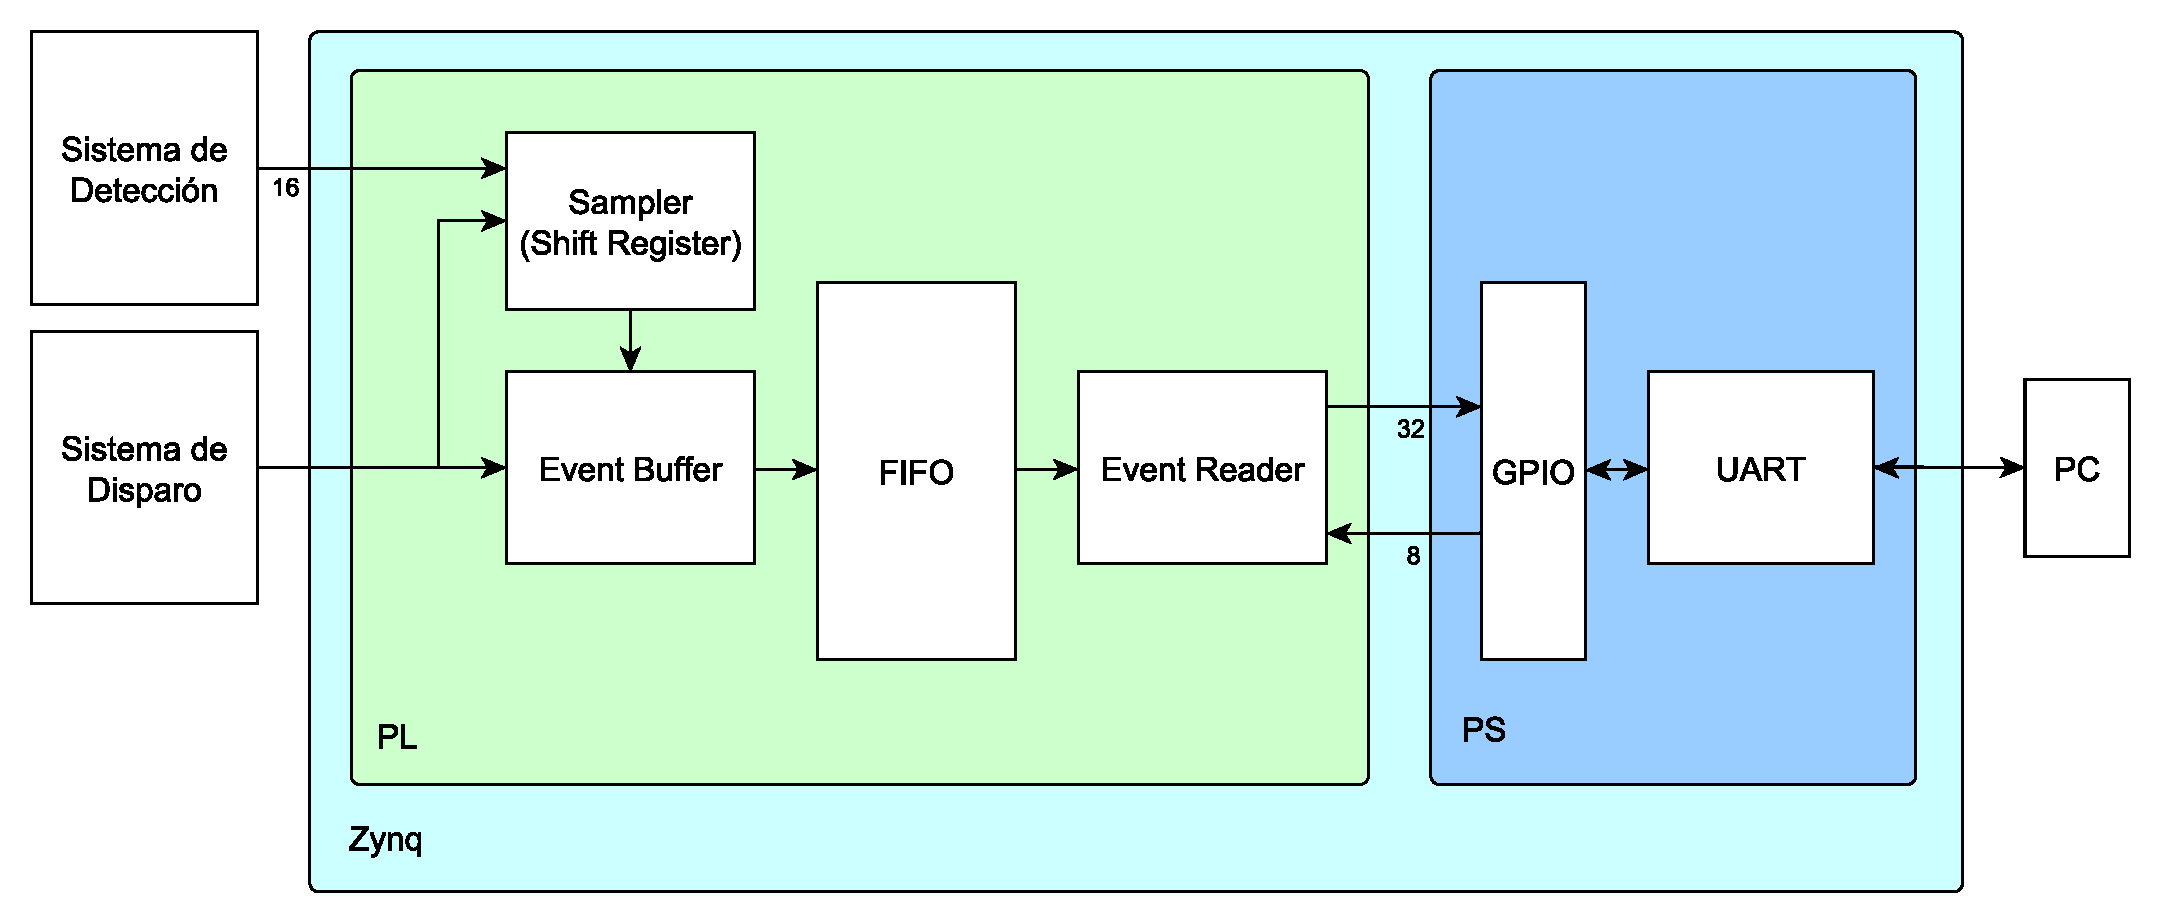
\includegraphics[scale=0.38]{muon-daq.pdf}
			\caption{Diagrama de la arquitectura de hardware propuesta para el diseño de un sistema de adquisición de datos asociado a un solo detector de muones.}
			\label{fig:muon-daq}
		\end{figure}
		
\section{Implementación del sistema de adquisición}
\label{sec:impl}
	La implementación del sistema de adquisición de datos en el módulo TE0720 se realizó mediante el software Vivado Design Suite 2019.1 y Vivado SDK 2019.1 para la descripción de hardware en lógica programable y  para la programación de software en el procesador, respectivamente. En esta sección se presenta el funcionamiento general de cada módulo y el detalle técnico de implementación se encuentra disponible en el repositorio Git\cite{GonzalezMuonRepository}. Adicionalmente, el Apéndice \ref{cap:git} instruye cómo utilizar Git como sistema de control de versiones para proyectos de descripción de Hardware Vivado como el desarrollado en esta memoria de titulación.
	
	La descripción de hardware se llevó a cabo en el HDL (Hardware Description Language) SystemVerilog y la integración de cada módulo se hizo mediante \textit{Block Design}, correspondiente a un método de descripción de hardware en formato de diagrama de bloques, el cual permite automatizar algunos procesos de instanciación de módulos e interconexión de puertos. En la Figura \ref{fig:blockdesign} se ilustra el diagrama de bloques del sistema de adquisición implementado en el módulo TE0720, donde se observan los diferentes bloques utilizados. El bloque \textit{ZYNQ7 Processing System} corresponde al procesador, donde se ubica el módulo de comunicación. El bloque \textit{top\_wrapper} agrupa los módulos \textit{Sampler, Event Reader y Event Buffer}, que junto con los bloques \textit{FIFO Generator}, \textit{Clocking Wizard} y \textit{clk\_divider} corresponden a los módulos implementados en la lógica programable. Los módulos \textit{AXI GPIO} corresponden a los puertos de entrada de datos y salida de comandos del sistema de comunicación incluido al interior del procesador, donde el módulo \textit{axi\_gpio\_0} está asociado a los 32bits de entrada de datos, mientras que el módulo \textit{axi\_gpio\_1} corresponde a los 8 bits de salida para comandos de lectura. Los bloques \textit{Processor System Reset} y \textit{AXI Interconnect} son módulos auxiliares instanciados de manera automática por el software y permiten generar las señales de \textit{reset} y habilitar la comunicación con la GPIO del procesador respectivamente. Por último, la señal \textit{trigger} corresponde a la señal de disparo, mientras que los arreglos de señales \textit{Ch\_A\_P[15:0]} y \textit{Ch\_A\_N[15:0]} corresponden a los puertos de entrada para las señales de detección LVDS con sus terminales positivos y negativos respectivamente.

	\begin{figure}[H]
		\centering
		\includegraphics[scale=0.4,angle=90]{blockdesignv2.png}
		\caption{Block Design del sistema de adquisición de datos implementado en el módulo TE0720.}
		\label{fig:blockdesign}
	\end{figure}
	
	A continuación se detalla del desarrollo de cada módulo, su funcionamiento, los puertos asociados, sus diagramas pertinentes y finalmente la utilización de hardware asociada a la totalidad del diseño implementado. \sgcnote{discutir detalles tecnicos una vez este entregado el informe.}
	
	\subsection{Sampler}
	\label{sec:sampling}
	
	El módulo \textit{Sampler} corresponde a la etapa de muestreo y discriminación, encargándose de recibir las señales digitales generadas por la interfaz ASD. Esta etapa muestrea cada señal entrante y asocia los datos a la señal de disparo correspondiente. Los principales objetivos de este módulo son:
	
	\begin{itemize}
		\item Muestrear los pulsos digitales la frecuencia lo más cercana a 600MHz (máxima frecuencia sintetizable en la plataforma de desarrollo Vivado, limitada por el IP Core \textit{Clocking Wizard}\cite{Xilinx2021ClockingSuite} \sgcnote{es un maximo indicado por fabricante? Una limitacion de los IPs?  Especificar}).
		\item Mantener en memoria los pulsos muestreados mientras llega la señal de disparo.
		\item Transferir los pulsos muestreados hacia la etapa siguiente al momento de detectar la señal de disparo.
	\end{itemize}

	Para interconectar la interfaz ASD con la tarjeta de desarrollo, se identificaron los conectores de cada dispositivo y se les asignaron etiquetas. Para el caso de la interfaz ASD se le asignó la letra ``A'' por ser la primera en ser conectada, nombrándose cada señal como ``JA-n'', donde ``n'' corresponde al número del pin de cada señal ubicada en el conector de 40 posiciones según la Tabla \ref{tab:asd-ports} \sgcnote{??} de la Sección \ref{sec:asd}.
	
	En el caso de la tarjeta de desarrollo Trenz TE0703, esta cuenta con dos conectores tipo VG96. La nomenclatura para cada pin se ilustra en la Figura \ref{fig:trenz-layout}, destacándose en verde los pines escogidos para interconectar la interfaz ASD. Estos pines se escogieron estratégicamente con el fin de estar ubicados en un extremo accesible, con puertos cercanos entre si, ordenados de manera consecutiva, y dejando espacio disponible para conectar otros detectores en el futuro.
	
	\begin{figure}[H]
		\centering
		\includegraphics[scale=0.7]{trenz-layout}
		\caption{Diagrama de la vista superior de la tarjeta de desarrollo utilizada, indicando la nomenclatura de los pines correspondientes a sus conectores VG96. Los pines utilizados para conectar la interfaz ASD se encuentran destacados en verde, enmarcados en el recuadro rojo.}
		\label{fig:trenz-layout}
	\end{figure}
	
	En la lógica programable, cada señal se recibe en los arreglo de puertos ``Ch\_A\_P[15:0]'' y ``Ch\_A\_N[15:0]'', donde ``Ch'' significa canal, ``A'' indica que corresponden la interfaz de lectura ``A'', ``P'' indica que son señales de polaridad positiva y ``N'' significa que son señales de polaridad negativa.
	
	En base a las nomenclaturas anteriores e incluyendo los propios nombres de los pines descritos en los esquemáticos eléctricos de la tarjeta de desarrollo TE0703\cite{TrenzElectronicGmbHTE0703SCH-TE0703-06} y los pines internos de la Zynq, se realizó la interconexión ASD-Zynq según lo indicado en la Tabla \ref{tab:zynq-asd} \sgcnote{Normalmente los caption de las tablas van sobre la tabla.}.
	
	\begin{table}[]
		\centering
		\caption{Mapeo de conexiones entre Zynq e interfaz ASD. }
		\resizebox{\textwidth}{!}{%
			\begin{tabular}{|c|c|c|c|c|c|}
				\hline
				\rowcolor[HTML]{4472C4} 
				\multicolumn{1}{|l|}{\cellcolor[HTML]{4472C4}{\color[HTML]{FFFFFF} \textbf{Zynq Pin}}} &
				\multicolumn{1}{l|}{\cellcolor[HTML]{4472C4}{\color[HTML]{FFFFFF} \textbf{Sch. Name}}} &
				\multicolumn{1}{l|}{\cellcolor[HTML]{4472C4}{\color[HTML]{FFFFFF} \textbf{Conn. VG96}}} &
				\multicolumn{1}{l|}{\cellcolor[HTML]{4472C4}{\color[HTML]{FFFFFF} \textbf{Conn. 40p ASD}}} &
				\multicolumn{1}{l|}{\cellcolor[HTML]{4472C4}{\color[HTML]{FFFFFF} \textbf{Channel}}} &
				\multicolumn{1}{l|}{\cellcolor[HTML]{4472C4}{\color[HTML]{FFFFFF} \textbf{Array}}} \\ \hline
				\rowcolor[HTML]{D9E1F2} 
				F16 & B35\_L1\_P  & J1-C2  & JA-9  & 0  & Ch\_A\_P{[}0{]}  \\ \hline
				E16 & B35\_L1\_N  & J1-C3  & JA-10 & 0  & Ch\_A\_N{[}0{]}  \\ \hline
				\rowcolor[HTML]{D9E1F2} 
				G17 & B35\_L6\_P  & J1-B3  & JA-11 & 1  & Ch\_A\_P{[}1{]}  \\ \hline
				F17 & B35\_L6\_N  & J1-B4  & JA-12 & 1  & Ch\_A\_N{[}1{]}  \\ \hline
				\rowcolor[HTML]{D9E1F2} 
				E15 & B35\_L3\_P  & J1-C4  & JA-13 & 2  & Ch\_A\_P{[}2{]}  \\ \hline
				D15 & B35\_L3\_N  & J1-C5  & JA-14 & 2  & Ch\_A\_N{[}2{]}  \\ \hline
				\rowcolor[HTML]{D9E1F2} 
				F18 & B35\_L5\_P  & J1-B5  & JA-15 & 3  & Ch\_A\_P{[}3{]}  \\ \hline
				E18 & B35\_L5\_N  & J1-B6  & JA-16 & 3  & Ch\_A\_N{[}3{]}  \\ \hline
				\rowcolor[HTML]{D9E1F2} 
				G19 & B35\_L20\_P & J1-C6  & JA-17 & 4  & Ch\_A\_P{[}4{]}  \\ \hline
				F19 & B35\_L20\_N & J1-C7  & JA-18 & 4  & Ch\_A\_N{[}4{]}  \\ \hline
				\rowcolor[HTML]{D9E1F2} 
				F21 & B35\_L23\_P & J1-B7  & JA-19 & 5  & Ch\_A\_P{[}5{]}  \\ \hline
				F22 & B35\_L23\_N & J1-B8  & JA-20 & 5  & Ch\_A\_N{[}5{]}  \\ \hline
				\rowcolor[HTML]{D9E1F2} 
				G15 & B35\_L4\_P  & J1-C8  & JA-21 & 6  & Ch\_A\_P{[}6{]}  \\ \hline
				G16 & B35\_L4\_N  & J1-C9  & JA-22 & 6  & Ch\_A\_N{[}6{]}  \\ \hline
				\rowcolor[HTML]{D9E1F2} 
				C17 & B35\_L11\_P & J1-B9  & JA-23 & 7  & Ch\_A\_P{[}7{]}  \\ \hline
				C18 & B35\_L11\_N & J1-B10 & JA-24 & 7  & Ch\_A\_N{[}7{]}  \\ \hline
				\rowcolor[HTML]{D9E1F2} 
				E19 & B35\_L21\_P & J1-C10 & JA-26 & 8  & Ch\_A\_P{[}8{]}  \\ \hline
				E20 & B35\_L21\_N & J1-C11 & JA-25 & 8  & Ch\_A\_N{[}8{]}  \\ \hline
				\rowcolor[HTML]{D9E1F2} 
				B16 & B35\_L8\_P  & J1-B11 & JA-27 & 9  & Ch\_A\_P{[}9{]}  \\ \hline
				B17 & B35\_L8\_N  & J1-B12 & JA-28 & 9  & Ch\_A\_N{[}9{]}  \\ \hline
				\rowcolor[HTML]{D9E1F2} 
				D16 & B35\_L2\_P  & J1-C12 & JA-29 & 10 & Ch\_A\_P{[}10{]} \\ \hline
				D17 & B35\_L2\_N  & J1-C13 & JA-30 & 10 & Ch\_A\_N{[}10{]} \\ \hline
				\rowcolor[HTML]{D9E1F2} 
				G20 & B35\_L22\_P & J1-B13 & JA-31 & 11 & Ch\_A\_P{[}11{]} \\ \hline
				G21 & B35\_L22\_N & J1-B14 & JA-32 & 11 & Ch\_A\_N{[}11{]} \\ \hline
				\rowcolor[HTML]{D9E1F2} 
				A21 & B35\_L15\_P & J1-C14 & JA-33 & 12 & Ch\_A\_P{[}12{]} \\ \hline
				A22 & B35\_L15\_N & J1-C15 & JA-34 & 12 & Ch\_A\_N{[}12{]} \\ \hline
				\rowcolor[HTML]{D9E1F2} 
				B21 & B35\_L18\_P & J1-B15 & JA-35 & 13 & Ch\_A\_P{[}13{]} \\ \hline
				B22 & B35\_L18\_N & J1-B16 & JA-36 & 13 & Ch\_A\_N{[}13{]} \\ \hline
				\rowcolor[HTML]{D9E1F2} 
				H22 & B35\_L24\_P & J1-C16 & JA-37 & 14 & Ch\_A\_P{[}14{]} \\ \hline
				G22 & B35\_L24\_N & J1-C17 & JA-38 & 14 & Ch\_A\_N{[}14{]} \\ \hline
				\rowcolor[HTML]{D9E1F2} 
				A18 & B35\_L10\_P & J1-B17 & JA-39 & 15 & Ch\_A\_P{[}15{]} \\ \hline
				A19 & B35\_L10\_N & J1-B18 & JA-40 & 15 & Ch\_A\_N{[}15{]} \\ \hline
			\end{tabular}%
		}
		\label{tab:zynq-asd}
	\end{table}
	
	Una vez definida la nomenclatura de puertos, es posible interconectar las tarjetas y proceder con la toma de muestras. Para capturar las señales LVDS, se declaran puertos IBUFDS (Input Buffer for Differential Signals) \cite{Xilinx2012XilinxDesigns} en la lógica programable, configurándolos para recibir señales LVDS de 2.5V y activando la resistencia interna de 100$\Omega$ para adaptar la terminación al estándar diferencial. Luego de ser capturar las señales LVDS\sgcnote{escritura}, estas se sincronizan con el reloj del circuito pasando a través de dos Flip-flops consecutivos (Synchonizer). En el Apéndice \ref{cap:lvds} se tratan más detalles relativos a la interconexión de puertos LVDS entre la interfaz ASD y productos de la familia Xilinx 7 Series.
	
	El muestreo de las señales se realiza a 400MHz por ser la frecuencia más alta sintetizable antes de producir errores de \textit{timing} en los períodos de \textit{setup} de señales asociadas a los módulos \textit{Sampler} y \textit{Event Buffer}, y en señales de alto \textit{fan-out} como la señal de reset del sistema completo (determinado experimentalmente siguiendo procedimientos y recomendaciones propias de la herramienta de diseño). La frecuencia de muestreo de 400MHz da una resolución de tiempo de 2,5ns para distinguir el ancho de los pulsos digitales, lo cual satisface los requerimientos descritos en la Sección \ref{sec:arq}.
	
	El método de muestreo utilizado consiste en un shift-register de 64 bits, el cual representa la ventana de adquisición del pulso digital capturado. Los 64 bits de este shift-register serán entregados a la siguiente etapa en el instante en que se reciba la señal de disparo. Considerando 16 canales con un buffer de 64 bits cada uno, el shift-register consiste en un arreglo bidimensional de 16 filas con 64 bits de ancho cada una.
	
	El shift-register funciona como buffer y retardo para la señal digital muestreada. Dada la frecuencia de muestreo, cada bit representa 2,5ns de la señal muestreada. Considerando que la señal de disparo posee un retardo de 100ns, a la llegada del disparo la señal queda ubicada entre el bit 24 y 63 aproximadamente. Esta configuración permite una ventana de 30ns antes de la señal de disparo y permite el muestreo de señales de hasta 130ns de duración. Se utiliza un shift-register debido a su simplicidad, su capacidad de operar a altas frecuencias de reloj y por permitir el almacenamiento natural por orden de llegada de cada bit digital de la la señal, haciendo posible entregar la totalidad de los datos contenidos en este shif-register a la etapa siguiente.
	
	Al detectar la señal de disparo, esta etapa registra los datos de todos los canales en un arreglo bidimensional y mantiene su estado hasta recibir la señal de que han sido guardados correctamente por la etapa siguiente. Mientras esto no suceda, el shift-register seguirá muestreando datos, pero se ignorarán las señales de disparo.
	
	La Figura \ref{fig:sampler} ilustra un diagrama simplificado del módulo \textit{Sampler} considerando la lógica para una sola señal LVDS entrante.
	
	\begin{figure}[H]
		\centering
		\includegraphics[scale=0.7]{sampler.pdf}
		\caption{Diagrama simplificado del módulo \textit{Sampler}, ejemplificado para una sola señal LVDS.}
		\label{fig:sampler}
	\end{figure}
	
	
	\subsection{Event Buffer}
	\label{sec:buffer}
	
	El buffer de eventos se encarga de almacenar provisoriamente los eventos entrantes en una memoria FIFO hasta que la etapa siguiente solicite la entrega de los eventos capturados. La frecuencia de operación escogida para el buffer es de 100MHz, facilitando la implementación de esta y las siguientes etapas al ser una de las frecuencias base de la tarjeta Trenz y por ser una frecuencia cerca de 600 veces más alta que el ratio de eventos detectados por minuto (1 evento por minuto en cada canal de detección). Operar el buffer de eventos a los 400MHz asociados a la etapa de muestreo requiere otras consideraciones de diseño, como por ejemplo implementar \textit{pipelines} y declarar \textit{constraints} de tiempo específicas para este propósito\cite{XilinxFIFOSuite}. \sgcnote{De donde viene esta limitacion? Esta indicado por el fabricante o es un tema de diseno?}
	
	Si se recibe una señal de disparo, el \textit{Event Buffer} procede a leer los datos provenientes de la etapa anterior (\textit{Sampler}). En cada ciclo de reloj se guarda en la memoria FIFO la última fila del arreglo bidimensional que representa al evento seleccionado. Una vez que la información es almacenada en memoria, se desplazan los datos del arreglo bidimensional (Shift) y se repite el ciclo 16 veces. Así, en la memoria FIFO cada dirección de memoria corresponderá a canales consecutivos de un mismo evento, donde cada canal es representado en 64 bits de datos. Se decidió operar de esta manera para simplificar la implementación del hardware y debido a que no es posible almacenar un arreglo bidimensional en una sola dirección de memoria FIFO. Además, se escogió una memoria FIFO para implementar este buffer por adecuarse bien a la naturaleza de los datos: el orden de los eventos es importante y con esta memoria los eventos son leídos por orden de llegada. Además, esta memoria permite el almacenamiento de mas de 50 eventos y sus respectivos canales.
	
	La Figura \ref{fig:event-buffer} ilustra el módulo \textit{Event Buffer} de manera simplificada, ejemplificando el flujo de información desde el evento seleccionado por el módulo \textit{Sampler} hasta la fila de 64bits a ser guardada en la memoria FIFO por cada ciclo de reloj hasta completar las 16 filas que componen el evento que está siendo guardado. Existe un contador que lleva la cuenta de las veces que se ha desplazado el arreglo bidimensional que contiene al evento y cuenta con lógica combinacional que coordina el flujo de la información. El módulo emite una señal para indicarle al módulo \textit{Sampler} que el evento ha sido guardado por completo en la memoria FIFO.
	
	\begin{figure}[H]
		\centering
		\includegraphics[scale=0.7]{event-buffer.pdf}
		\caption{Diagrama simplificado del módulo \textit{Event Buffer}.}
		\label{fig:event-buffer}
	\end{figure}
	
	\subsection{Event Reader y Comunicación}
	\label{sec:comm}
	El módulo \textit{Event Reader}, ilustrado en el costado izquierdo de la Figura \ref{fig:com} cumple la función de leer los eventos almacenados en la memoria FIFO cada vez que reciba un comando de 8 bits desde el módulo de comunicación. Al recibir el comando, el módulo comienza a leer cada dirección de la memoria FIFO hasta leer las 16 direcciones consecutivas que componen a un mismo evento. Cada dirección almacena un canal de detección en 64bits, pero el \textit{Event Reader} separa esta información en 2 paquetes de 32bits cada uno, demorando dos ciclos de reloj por cada canal que se desee enviar. Este formato de entrega permite la comunicación entre la lógica programable y el procesador mediante el GPIO, utilizando un puerto de precisamente 32bits. Dado que el GPIO del procesador cuenta con puertos limitados, no es posible utilizar un puerto de 64Bits de manera directa, debiendo realizarse en dos pasos. Por otro lado, los datos se entregan desde la PL al PS y no al revés debido a que el módulo de comunicación UART (Universal Asynchronous Receiver-Transmitter) está ubicado en el procesador, mientras que los datos están almacenados en la lógica programable.
	 
	Complementariamente, la etapa de comunicación ilustrada en el costado derecho de la Figura \ref{fig:com} se encarga de entregar los eventos recibidos desde el \textit{event reader} hacia el mundo exterior mediante la UART presente el procesador de la Zynq, a una tasa de transferencia de 115.200bps (baudios por segundo). Este módulo recibe comandos en formato ASCII desde un computador externo (que serán traspasados al módulo \textit{Event Reader}) y entrega los datos provenientes de la lógica programable al computador solicitante en forma de números enteros sin signo de 32bits.
	
	\begin{figure}[H]
		\centering
		\includegraphics[scale=0.67]{com.pdf}
		\caption{Diagrama simplificado del módulo \textit{Event Reader} y el módulo de comunicación en el procesador.}
		\label{fig:com}
	\end{figure}
	
	\sgcnote{Se hizo mencion al repositorio en caso de que se quieran ver mas detalles Esto ayudaria a darle mas fuerza al trabajo, y que no quede como que dijiste que lo hiciste, pero no hay pruebas.}\sjgnote{Asi es, lo menciono al inicio de la seccion de implementacion}
	
	\subsection{Utilización de recursos en el sistema implementado}
	
	La implementación de este sistema de adquisición significó la utilización de casi 23\% de la memoria BRAM disponible para la implementación del módulo \textit{Event Buffer}, como se indica en la Tabla \ref{tab:resources}. Se utilizaron 32 bloques de 36Kb cada uno para la implementación de la memoria FIFO asociada a los eventos provenientes de un detector. Sumado a que se utilizaron 33 puertos IO (32 puertos para señales LVDS y 1 para la señal de disparo) de los 152 accesibles desde la tarjeta de desarrollo Trenz, se tiene que el uso de recursos es menor al 25\% y da pie para implementar un sistema de adquisición para máximo 4 detectores antes de utilizar la totalidad de recursos de memoria disponibles.
	
	En cuanto a otros recursos utilizados listados en la Tabla \ref{tab:resources}, se usa un solo MMCM (Mixed-mode Clock Manager) y 3 BUFG (Global Clock Buffer) para la generación de relojes, no debiendo requerirse MMCM adicionales en una eventual expansión del sistema de adquisición dentro del mismo hardware. La utilización de Flip-flops representa aproximadamente un 6\% del total disponible, lo que corresponde a un bajo porcentaje de utilización considerando que son el principal recurso de hardware presente en el muestreo de señales digitales y en la escritura y lectura de eventos en memoria, significando una ventaja y abriendo la posibilidad a expandir la lógica programable. Así mismo, los porcentajes de utilización asociados a LUTs (Look-up Tables) y memoria distribuida (LUTRAM) presentes en la lógica combinacional son mínimos comparado con el total disponible, lo que da holgura para implementar sistemas aún más grandes y complejos.
	
	Luego de la implementación y análisis del sistema de adquisición de datos diseñado, es posible operar el sistema y capturar pulsos de prueba, leer los datos muestreados y contrastar la integridad de la información entre los pulsos iniciales y los datos leídos por comunicación serial como se realizará en el Capitulo \ref{cap:sim}.
	
	\begin{table}[]
		\centering
		\caption{Recursos de hardware utilizados en la implementación del sistema de adquisición.}
		\label{tab:resources}
		\begin{tabular}{lrrr}
			\hline
			\textbf{Recurso} & \multicolumn{1}{l}{\textbf{Utilización}} & \multicolumn{1}{l}{\textbf{Disponibilidad}} & \multicolumn{1}{l}{\textbf{Utilización {[}\%{]}}} \\ \hline
			LUT    & 2.810 & 53.200  & 5,28  \\
			LUTRAM & 80    & 17.400  & 0,46  \\
			FF     & 6.439 & 106.400 & 6,05  \\
			BRAM   & 32    & 140     & 22,86 \\
			IO     & 33    & 200     & 16,50 \\
			BUFG   & 3     & 32      & 9,38  \\
			MMCM   & 1     & 4       & 25,00   
		\end{tabular}
	\end{table}

\newpage
\thispagestyle{empty}
\cleardoublepage

\chapter{simulaciones}
\label{cap:sim}
Con el fin de poner a prueba el hardware diseñado, se proponen dos tipos de pruebas. 
La primera prueba consiste en generar pulsos digitales de duración conocida y capturarlos directamente en los puertos de entrada del circuito.

La segunda prueba consiste en generar pulsos analógicos de carga conocida y capturarlos con la interfaz ASD. Esta estará conectada a los puertos del hardware diseñado.

\section{Pulsos digitales
explicacion

objetivos

disposicion experimental, recursos utilizados, metodo

resultados

conclusiones, datos, graficos
}

\section{Pulsos analógicos}

explicacion

objetivos

disposicion experimental, recursos utilizados, metodo

resultados

conclusiones, datos, graficos


\newpage
\thispagestyle{empty}
\cleardoublepage

\chapter{conclusion}
\label{cap:conclusiones}
\gcnote{Falta un parrafo introductorio sobre lo que se trata en este capitulo. Cada capitulo debe tener uno.}

\section{Conclusiones}
\label{sec:conc}

Luego del trabajo realizado en esta memoria de titulación se logró cumplir con los objetivos propuestos en la Sección \ref{sec:planteamiento}. Fue posible diseñar e implementar un sistema digital capaz de cumplir con las funciones de adquirir pulsos digitales proveniente de una interfaz de lectura, discriminar la autenticidad de los eventos capturados asociados a muones y comunicar los datos adquiridos a sistemas externos, todo implementado en una tarjeta de desarrollo Trenz consistente en un SoC Zynq 7000 constituido por un procesador y lógica programable equivalente a la de una FPGA Artix 7. Las etapas de adquisición y discriminación lograron implementarse con buffers de entrada para señales LVDS y Shif-registers respectivamente, mientras que la etapa de comunicación se llevó a cabo utilizando una memoria FIFO y comunicación serial implementada en el procesador de la tarjeta Trenz.

Fue posible realizar un diseño escalable mediante el la creación de un sistema modular basado en etapas de adquisición de datos, escritura y lectura de memoria. Dado que la tarjeta Trenz cuenta con 76 pares de puertos compatibles con el estándar LVDS y con 4.9Mb de memoria distribuida en 140 bloques de 36Kb cada uno, es posible implementar con holgura dos sistemas de adquisición en una misma tarjeta, utilizando 32 puertos LVDS, 1 puerto común para señal de disparo y capacidad de almacenar hasta 2.500 eventos. Utilizando los recursos al límite, es factible implementar 4 sistemas de adquisición en una misma tarjeta Trenz, pero reduciendo la cantidad de eventos almacenables a 1.250 antes de llenar por completo la memoria FIFO. Esto no es un problema mientras los datos sean leídos de manera constante o al menos cada 1 minuto, ya que el flujo de muones en el área de detección asociada a 4 detectores corresponde a 900 eventos por minuto, llenando la memoria totalmente en cerca de minuto y medio.

La resolución espacial alcanzada por el detector es efectivamente de 1cm$^2$ mediante el cruce de canales excitados por señales de detección según el esquema de coordenadas indicado en la Figura \ref{img:cuadrantes-ministgc} de la Sección \ref{sec:stgc}. Esta resolución puede mejorar considerablemente mediante un posterior análisis de duración de pulsos detectados en canales adyacentes al vértice de interacción estimado. 

Por otro lado, la resolución temporal del sistema de adquisición diseñado fue de 2,5ns, dentro del rango de los nanosegundos, gracias a la frecuencia de reloj de 400MHz utilizada en la etapa de muestreo. Si bien esta resolución cumple con los requisitos, no es la máxima factible a sintetizar en la lógica programable de la tarjeta Trenz. Para lograr mayores frecuencias de reloj es necesario cambiar el esquema de comunicación entre los módulos de muestreo y buffer de eventos, ya que pertenecen a dominios de reloj diferentes. En un principio, se trabajó sin darle importancia a los dominios de reloj asociados a cada módulo para simplificar el diseño de hardware cumpliendo con los requerimientos de tiempo establecidos, pero durante el desarrollo del sistema de adquisición se tornó evidente la necesidad de implementar una memoria de doble puerto con operación de relojes independientes para permitir una comunicación óptima entre módulos a una frecuencia mayor. También es posible cambiar la manera en que se resetean algunos bloques lógicos, sobre todo aquellos encargados de retener la información de los eventos, logrando tener un \textit{fanout} mucho menor en las señales de reset utilizadas, evitando por ejemplo el restablecimiento de algunos arreglos bidimensionales y dependiendo solo de su inicialización y flujo en las máquinas de estados, tema que no fue considerado al momento de diseñar el sistema de adquisición. Para alcanzar frecuencias de muestreo aún mayores, sería necesario cambiar a plataformas híbridas de adquisición de datos, como por ejemplo utilizando FPGAs en conjunto con chips DRS4\cite{RittDRS4Array} alcanzando tasas de muestreo equivalentes a utilizar un reloj de 5GHz para el caso de esta memoria. Sin embargo, frecuencias por sobre 1GHz no se justifican para la aplicación en sTGC minería, principalmente por la resolución temporal de la tarjeta ASD (no mayor a 1ns).

El haber superado satisfactoriamente la prueba experimental con pulsos digitales emulados sienta precedentes satisfactorios para una posterior prueba con interfaces ASD reales y con detectores sTGC funcionales. La totalidad %\sgcnote{pero el 100\% de lo que hiciste es 100\% representativo de lo que pasaria en la practica? Si envie 1 dato y lo recibi, tambien podria decir que tuve un 100\% de exito.}
de los datos emulados fue muestreado con la resolución temporal esperada, implicando que la existencia de eventos defectuosos es menor al 1\% y asegurando una resolución temporal de $\pm$2,5ns para la duración de las señales muestreadas. Se espera que las tasas de error alcanzadas dentro del sistema de adquisición sean las mismas al probar el sistema con eventos reales, pero podrían presentarse otros errores no considerados en los sistemas de disparo y detección que podrían contribuir al alza de la tasa de error y a la reducción de la resolución temporal de sTGC Minería en su totalidad.


Por último, el trabajo realizado, los sistemas estudiados y las herramientas utilizadas se encuentran disponibles en la enciclopedia digital de CCTVal, así como también en el repositorio de Github \cite{GonzalezMuonRepository}, permitiendo la replicación, mejoramiento y continuación de este proyecto, así como también la oportunidad de adaptarlo a otros sistemas que requieran adquisición de datos en su arquitectura.


\section{Trabajo Futuro}

Para el futuro quedan pendientes muchas opciones de desarrollo interesantes. Por ejemplo, es posible fabricar una tarjeta PCB (Printed Circuit Board) que facilite la interconexión de las interfaces de lectura hacia la tarjeta Trenz. Esta PCB deberá cumplir con el estándar LVDS para señales diferenciales tomando en consideración la simetría e impedancia presente en las pistas que la compongan. Por otro lado, queda pendiente seguir mejorando el diseño digital del sistema de adquisición, poniendo al límite sus posibilidades para mejorar el desempeño en cuanto a resolución temporal. Como se menciona en la Sección \ref{sec:conc} inmediatamente anterior, es factible repensar la comunicación entre distintos dominios de reloj y optimizar la utilización de señales con alta demanda, como lo son las señales de reloj y reset. Además, es posible abarcar nuevos métodos de optimización \textit{post-placement} mediante comandos y análisis de \textit{timing}\cite{XilinxUltraFastGuide} propios de la herramienta de diseño Vivado, que podrían ayudar a alcanzar al menos los 500MHz de frecuencia de reloj.

Finalmente, queda pendiente la realización de pruebas mediante pulsos analógicos provenientes de generadores de señales y circuitos adecuados para estos fines. Además, se deberá probar el sistema con interfaces ASD reales y conectadas a sus respectivos detectores para así caracterizar el sistema completo y observar las propiedades físicas de los muones detectados. Queda pendiente también interconectar este proyecto con el sistema de disparo\cite{Oyanadel2020SistemaSTGC} fabricado por CCTVal en conjunto con el detector y la interfaz de lectura, completando así la primera etapa del proyecto sTGC Minería. Una segunda futura etapa, posterior a la adquisición de datos para detectores de muones, será la etapa de análisis de datos para reconstrucción de eventos de detección, encargada de interpretar la duración de los pulsos capturados asociados a los diferentes canales de detección. Este análisis de datos permitiría el estudio de la posición y la energía depositada por los muones en los detectores, estimar la trayectoria de los muones y determinar la densidad de la materia atravesada en su camino, logrando así generar las tomografías muónicas útiles para el estudio de terreno minero, tal como se requiere en el proyecto sTGC Minería de CCTVal.


\newpage
\thispagestyle{empty}
\cleardoublepage


%%%------------------APÉNDICES--------------------------------

\appendix
\chapter{Conexión de señales LVDS en Familia de Productos Xilinx 7 Series}
\label{cap:lvds}
Este proyecto basa su funcionalidad en un enlace de datos físicos ente una FPGA y una interfaz de lectura ASD, en donde la interfaz emite pulsos digitales através de emisores LVDS internos y FPGA recibe los pulsos mediante un receptor interno. Este apéndice detalla cómo interconectar dispositivos que utilicen interfaces LVDS en cualquier tipo de proyecto, entendiendo los protocolos y requerimientos necesarios para lograrlo.

\section{Acerca del estándar LVDS}	
	LVDS (Low Voltage Differential Signaling) es un enlace de datos de capa física, útiles en aplicaciones que requieran principalmente conservar la integridad de los datos, mantener bajo ruido en el medio de transmisión, o cuando el emisor y receptor se encuentran demasiado lejos el uno del otro.
	
\section{Características principales}
	
	Las interfaces LVDS pueden controlar señales en el rango de los 2V a 5V, con una alta velocidad de transferencia de hasta 500Mbps en un solo par diferencial preservando la integridad de la señal a transmitir y manteniendo una buena inmunidad al ruido y a interferencia por campos electromagnéticos Se caracterizan por ser económicas, de bajo consumo de potencia, pequeñas y de una implementación simple.

	Las interfaces LVDS transfieren datos a través de una linea de par trenzado en la que los voltajes de cada alambre tienen opuesta amplitud de voltaje. Estas señales son montadas sobre un nivel de voltaje continuo típicamente de 1,2V y poseen tan solo 400mV de diferencia de voltaje ente ambos alambres. La Figura IMAGE ilustra estos niveles de voltaje.
	
	La Figura IMAGE ilustra las señales LVDS, mostrando primero una señal de una linea para luego ilustrar la señal diferencial en sí misma. V$_{idth}$ (Input Differential Threshold Voltage) corresponde al nivel de voltaje después de que el receptor capura la señal diferencial entrante.  V$_{ob}$ corresponde al alambre con potencial de voltaje positivo,  V$_{oa}$ corresponde al alambre de potencial negativo y  V$_{od}$ representa la diferencia de voltaje final ente el par de alambres.
	
	Los las interfaces diferenciales solamente emiten y reciben la diferencia entre los dos alambre que componen la linea de transmisión, eliminando el ruido de modo común en la señal de voltaje asociado a la diferencia de voltaje existente entre la tierra eléctrica , el emisor y el receptor, sumado al ruido propio infiltrado en la linea de transmisión.
	
	La implementación de una linea de datos LVDS requiere un emisor, una linea de transmisión, un resistor de 100$\Omega$ y un receptor, como se observa en la Figura IMAGE. El resistor de 100$\Omega$ se debe a la impedancia propia de la linea de transmisión (50$\Omega$) de cada alambre respecto a tierra, junto a una linea de transmisión simétrica se obtiene un medio de comunicación que mantiene la adaptación de impedancia y la integridad de la señal enviada. 


\section{Interconexión LVDS para hardware Xilinx Series 7}

	La familia de FPGAS Xilinx 7 series son capaces de operar con señales LVDS tanto en su emisión como recepción, con la opción de habilitar un resistor de 100$\Omega$ en caso de que el circuito conectado no cuente con él. Además, esta familia de FPGAS cuenta con dos tipos de estándar LVDS, el LVDS común que requiere una fuente de 1.8V y se encuentra disponible en los bancos HP (High Performance) de la FPGA, y el están LVDS\_25, el cual necesita una fuente de voltaje de 2,5V para alimentar sus bancos de puertos correspondientes unicamente a los de tipo HR (High Rank). Usar cualquiera de estos dos estándares con su correcta fuente de voltaje permita habilitar o deshabilitar el resistor interno, de lo contrario, en el caso de usar un voltaje diferente se debe mantener el resistor interno desactivado.
	
	En particular, la FPGA Artix 7 y la Zynq 7000 tienen solamente bancos HR, por lo que solo está disponible el estándar LVDS\_25, pero las tarjetas Trenz utilizadas en esta memoria de titulación solo cuentan con fuentes de 1,8V, 3,3V y 5V, lo que implica que para utilizar el resistor interno se debe utilizar una fuente de voltaje externa de 2,5V

\section{Descripción de hardware para utilización de puertos LVDS}

	Para operar correctamente utilizando puertos LVDS en la familia de FPGAs Xilinx 7 series es necesario declarar los puertos a utilizar y el voltaje asociado en el archivo de \textit{constraints} XDC. Por ejemplo para utilizar el par diferencial B16\_L22\_P (positivo) y B16\_L22\_N (negativo) ubicados respectivamente en los puertos E22 y D22 de la FPGA, se declararían las siguientes lineas:
	
	CODIGO

%set_property -dict {PACKAGE_PIN E22 IOSTANDARD LVDS_25} [get_ports B16_L22_P];
%set_property -dict {PACKAGE_PIN D22 IOSTANDARD LVDS_25} [get_ports B16_L22_N];

	Finalmente, para poder utilizar correctamente el par diferencial, es necesario utilizar un \textit{IO Buffer} instanciado en el hardware descrito. Estos buffers permiten convertir la señal diferencial a una de un solo terminal o viceversa. Por ejemplo, para usar un par diferencial según el estándar LVDS\_25 habilitando la resistencia interna del puerto, bastaria con declarar un IBUFDS (Input Buffer for Differential Singal) como se indica a continuación:
	
	CODIGO:


%// IBUFDS: Differential Input Buffer - Verilog
%// 7 Series
%// Xilinx HDL Libraries Guide, version 13.4
%IBUFDS #(
%    .DIFF_TERM("TRUE"), // Differential Termination (TRUE or FALSE)
%    .IBUF_LOW_PWR("FALSE"), // Low power="TRUE", Highest performance="FALSE"
%    .IOSTANDARD("LVDS_25") // Specify the input I/O standard (LVDS or LVDS_25)
%    ) IBUFDS_LVDS_25 (
%    .O(lvds_output), // Buffer output
%    .I(B16_L22_P), // Diff_p buffer input (connect directly to top-level port)
%    .IB(B16_L22_N) // Diff_n buffer input (connect directly to top-level port)
%);
%// End of IBUFDS_inst instantiation

Siguiendo estos pasos, el receptor LVDS queda correctamente configurado. Para utilizar el receptor basta con conectar las respectivas señales diferenciales en los puertos correspondientes declarados en el diseño y utilizar un cable de par trenzado simétrico con una impedencia de 50$\Omega$.

\chapter{Control de versiones de proyectos Vivado con Git}
\label{cap:git}
\textit{Git} es un sistema de control de versiones que permite al desarrollador crear múltiples ramas de desarrollo, sincronizar su trabajo con otros desarrolladores, revertir cambios realizados en el código y mantener una versión ordenada de un proyecto. Usar este tipo de herramientas para el desarrollo de proyectos en Vivado Desing Suite resulta ser muy útil, ya que permite trabajar de manera colaborativa y llevar registro de las versiones del hardware diseñado. En este apéndice se resumen todos los consejos y etapas para llevar a cabo el control de versiones de un proyecto Vivado. La clave del método a describir consiste subir al repositorio solo los archivos principales del proyecto, dejando fuera cualquier otro archivo proveniente de etapas de síntesis, implementación o archivos generados automáticamente por Vivado. Para llevar a cabo el control de versiones se hace uso de \textit{git} junto con la plataforma en línea \textit{Github.com}.

Antes de comenzar, se debe contar con los siguientes requisitos:
\begin{itemize}
	\item Nociones básicas de \textit{git}.
	\item Una cuenta en \textit{Github.com}.
	\item El software de control de versiones \textit{git} instalado en el computador y habilitado para ser operado mediante un terminal de comandos.
	\item Tener instalado Vivado Design Suite (La versión utilizada en este tutorial corresponde a la versión 2019.1).
\end{itemize}

\section{Creación de un repositorio Git}

	Para comenzar, se debe iniciar sesión en \textit{Github.com} y hacer clic en el botón verde  ``New'' ubicado en la esquina superior izquierda, como se ilustra en la Figura \ref{fig:git1}.
	
	\begin{figure}[ht]
		\centering
		\includegraphics[scale=0.6]{git1.png}
		\caption{Botón ``New'' para la creación de un nuevo repositorio remoto en \textit{Github.com}.}
		\label{fig:git1}
	\end{figure}
	
	Se debe elegir el nombre del repositorio y configurar lo esencial. Se recomienda crear un proyecto en blanco, sin archivo \textit{readme} o \textit{.gitignore}, ya que serán subidos al repositorio de manera remota durante el primer \textit{commit}.

\section{Clonación de un repositorio Git}

	Desde la interfaz web del repositorio de Github.com debe buscarse el botón verde llamado ``Code'' (ubicado en la esquina superior derecha) y copiar en el portapapeles la \textit{URL} disponible para clonar el repositorio mediante HTTPS (Hypertext Transfer Protocol Secure), como se ilustra en la Figura \ref{fig:git2}.
	
	\begin{figure}[ht]
		\centering
		\includegraphics[scale=0.5]{git2.png}
		\caption{Botón ``Code'' para acceder al enlace de clonación del repositorio.}
		\label{fig:git2}
	\end{figure}
	
	Si aún no se tiene instalado \textit{git} en el computador, se debe proceder a su instalación vía consola o mediante descarga directa. Luego, se debe acceder o crear una carpeta para guardar el repositorio Vivado, abrir en ella una consola de comandos y escribir lo siguiente, sustituyendo \textit{your-git-url} con el enlace copiado en el portapapeles:

\begin{lstlisting}[language=bash]
$ git clone your-git-url
\end{lstlisting}


\section{Creación de los archivos y carpetas iniciales}

	Para crear los primeros archivos del repositorio se debe acceder a la carpeta escogida y crear 5 nuevas carpetas en su interior llamadas \textit{ip}, \textit{src},  \textit{sim}, \textit{xdc} y \textit{wd}.
	
	\begin{itemize}
		\item \textit{ip}: Esta carpeta incluirá los archivos asociados a IP Cores.
		\item \textit{src}: Esta carpeta es la indicada para guardar los archivos de código HDL.
		\item \textit{sim}: Carpeta para almacenar \textit{testbenchs}.
		\item \textit{xdc}: Carpeta destinada a guardar archivos XDC para \textit{constraints} y declaraciones de puertos.
		\item \textit{wd}: Esta carpeta es la indicada para guardar los archivos generados automáticamente por Vivado durante las etapas de síntesis e implementación. Esta carpeta no debe ser incluida en los \textit{commits} de \textit{git}, ya que contiene precisamente la información que no requiere seguimiento en el repositorio.	
	\end{itemize}
	
	Luego, se puede crear un archivo \textit{README.md} y uno \textit{.gitinit} en la carpeta principal. El archivo \textit{README.md} es relevante para explicar el contenido del repositorio y debe ser escrito en lenguaje \textit{Markdown}. En el archivo \textit{.gitinit} se deben incluir todos los formatos de archivo que no quieran ser subidos al repositorio, como lo son los archivos creados automáticamente por el sistema o la carpeta \textit{wd} mencionada anteriormente. Se sugiere agregar las siguientes lineas en este archivo \textit{.gitinit}:

\begin{lstlisting}[language=bash, frame=single]
wd/
.Xil/
\end{lstlisting}

\section{Preparación del proyecto Vivado}
	Antes que todo, se debe crear un proyecto Vivado y guardarlo en la carpeta \textit{wd} anteriormente creada. Si el proyecto ya existía, entonces basta con trasladar el proyecto completo y guardarlo al interior de la carpeta \textit{wd}. Luego de ello, se deben copiar o crear los archivos fuente del diseño en HDL, los archivos de simulación y los \textit{constraints} en sus respectivas carpetas.
	
	Si el diseño de hardware utiliza IP Cores, hay que asegurarse de habilitar la opción de \textit{IP Core Containers} en Vivado. Esta opción se encuentra en el menú \textit{Tools$>$ Settings$> $Project Settings$>$ IP$>$ Core Containers: Use Core Containers for IP} ilustrado en la Figura \ref{fig:viv1}, lo que facilita el control de versiones creando un solo archivo \textit{.xcix} que contiene al IP Core en su totalidad. Si Vivado pregunta por convertir el IP Core actual a un \textit{container}, dar clic en \textit{OK} y mover los \textit{containters} a la carpeta \textit{ip} correspondiente en el repositorio.
	
	\begin{figure}[ht]
		\centering
		\includegraphics[scale=0.5]{viv1.png}
		\caption{Menú de configuración para la habilitación de IP Containers en Vivado.}
		\label{fig:viv1}
	\end{figure}
	
	Finalmente, se deben importar los archivos contenidos en las carpetas \textit{src, sim, xdc} e \textit{ip} al proyecto de descripción de hardware en la vista \textit{Project Manager} de Vivado.

\section{Exportar script Tcl}

	Desde la interfaz de Vivado se debe exportar el archivo \textit{Tcl} (Tool Command Language) asociado al proyecto Vivado accediendo a \textit{File$>$ Project$>$ Write Tcl} ilustrado en la Figura \ref{fig:viv2} y guardándolo con el nombre \textit{build.tcl} en la carpeta principal de repositorio, no en las subcarpetas creadas. Se debe tener encuentra que el proceso de exportación y edición del archivo Tcl debe realizarse cada vez que se crea o elimina un nuevo archivo fuente del proyecto. En caso de no realizar la exportación, el script no generará el proyecto completo y habrá que importar los archivos fuente de manera manual.
	
	\begin{figure}[ht]
		\centering
		\includegraphics[scale=0.6]{viv2.png}
		\caption{Ventana de Vivado para la exportación de un script Tcl.}
		\label{fig:viv2}
	\end{figure}

\section{Editar script Tcl}
	Un paso importante en este proceso de control de versiones es la edición del archivo Tcl, para que así se generen automáticamente los archivos de Vivado en la carpeta \textit{wd}. Para lograrlo, se debe abrir el archivo \textit{build.tcl} en un editor de texto y buscar los siguientes comandos:

\begin{lstlisting}[language=bash, frame=single, basicstyle=\small]
	
# Set the reference directory for source file relative paths 
#(by default the value is script directory path)
set origin_dir "."

# Set the directory path for the original project from where
#this script was exported
set orig_proj_dir "path-to-the-actual-vivado-project"
	
# Create project
create_project ${_xil_proj_name_} ./${_xil_proj_name_} 
	-part part-of-your-fpga

\end{lstlisting}

	Una vez ubicados, se deben reemplazar por los siguientes comandos:
	
\begin{lstlisting}[language=bash, frame=single, basicstyle=\small]
	
# Set the reference directory for source file relative paths 
#(by default the value is script directory path)
set origin_dir [file dirname [info script]]

# Set the directory path for the original project from where 
#this script was exported
set orig_proj_dir "[file normalize "$origin_dir/wd/"]"

# Create project
create_project ${_xil_proj_name_} $orig_proj_dir/${_xil_proj_name_} 
	-part part-of-your-fpga

\end{lstlisting}


\section{Confirmar y subir los archivos al repositorio remoto}

	En este punto todo se encuentra listo para realizar el primer \textit{commit} en \textit{git} y comenzar el control de versiones del proyecto Vivado mediante el siguiente comando en consola:
	
\begin{lstlisting}[language=bash, frame=single]
$ git add .
$ git commit -m "First commit."
$ git push

\end{lstlisting}

	Luego de ejecutar los comandos en consola, el control de versiones se encuentra correctamente configurado y es seguro eliminar el proyecto Vivado de otras ubicaciones fuera del repositorio, ya que el proyecto puede ser reconstruido completamente al ejecutar el script \textit{ build.tcl} desde la consola Tcl de Vivado.




%%%%%%%%%%%%%%%%%%%%%%%%%%%%%%%%%%%%%%%%%%%%%%%%%%%%%%%%%%%%%%%%%%%%%%%%%%%%%%%%%%
%%%------------------BIBLIOGRAFÍA-----------------------------

\bibliographystyle{IEEEtran}
\bibliography{references}

\end{document}







